\chapter{Complex Components}

\section{Axial Power Transmission}

Getting power transmitted over a shaft in a straight line is not terribly difficult, but still must be done properly.

\subsection{Shafts, Hubs, and Interfaces}
	
	\textit{Shafts}\index{shafts} or \textit{axles}\index{axles} are rotating components which mate into \textit{hubs}. \textit{Hubs}\index{hubs} may be used then to mount to other useful components like wheels or arms, or may be integral to said useful components.

	\begin{figure}[H]
		\centering
		\begin{subfigure}[b]{.32\linewidth}
			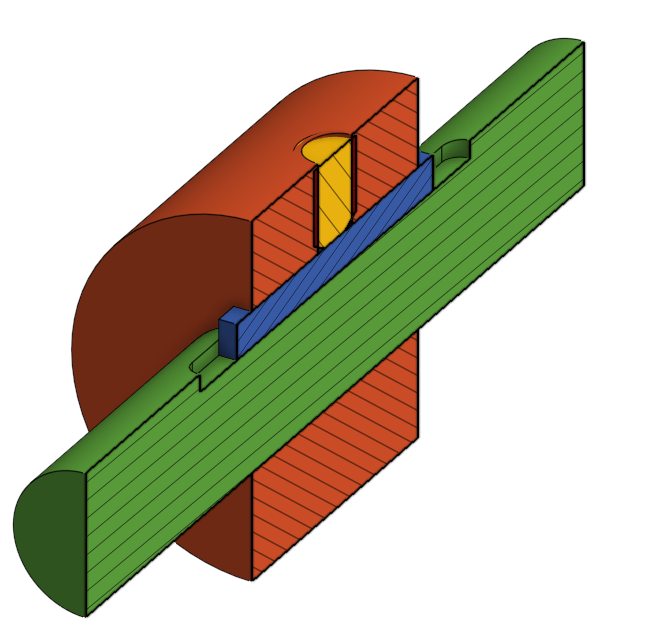
\includegraphics[width=0.6\textwidth]{imgs/keyedshaft.png}
			\caption{Keyway with set screw}
		\end{subfigure}
		\begin{subfigure}[b]{.32\linewidth}
			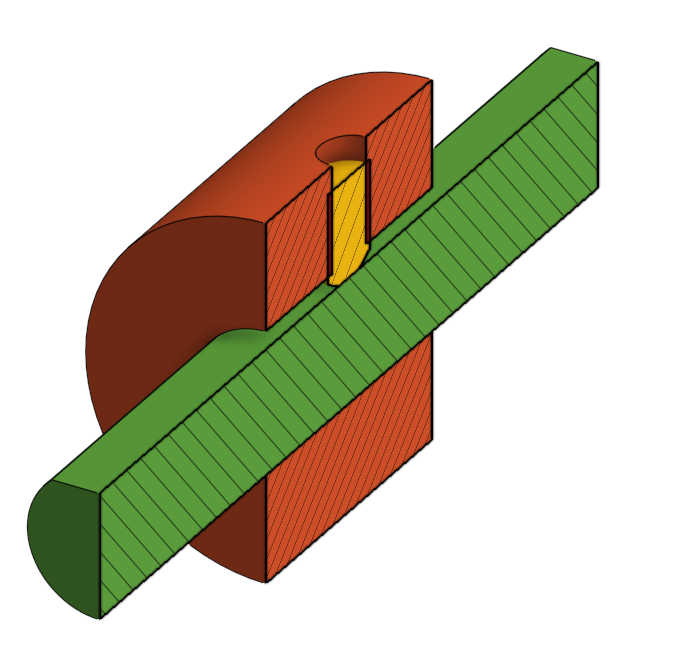
\includegraphics[width=0.6\textwidth]{imgs/dshaft.png}
			\caption{D-shaft with set screw}
		\end{subfigure}
		\begin{subfigure}[b]{.32\linewidth}
			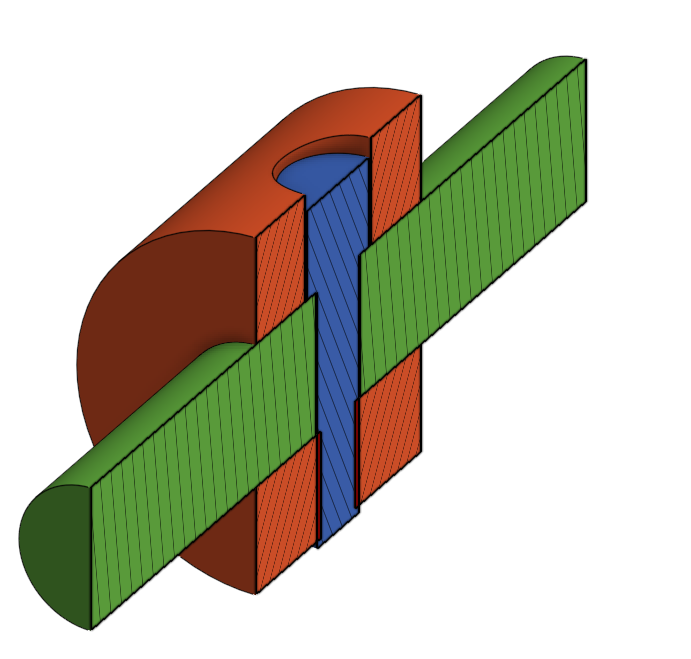
\includegraphics[width=0.6\textwidth]{imgs/pinnedshaft.png}
			\caption{Pinned}
		\end{subfigure}
		\begin{subfigure}[b]{.32\linewidth}
			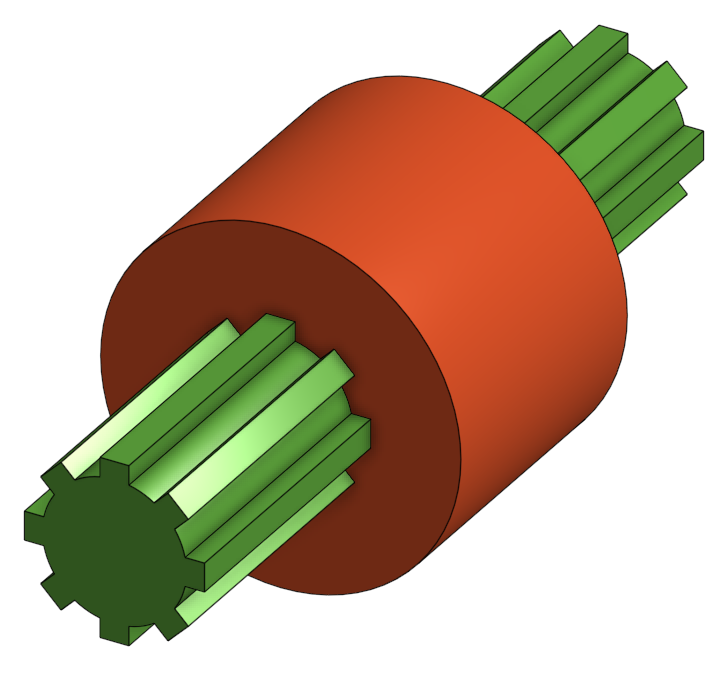
\includegraphics[width=0.6\textwidth]{imgs/splineshaft.png}
			\caption{Spline}
		\end{subfigure}
		\begin{subfigure}[b]{.32\linewidth}
			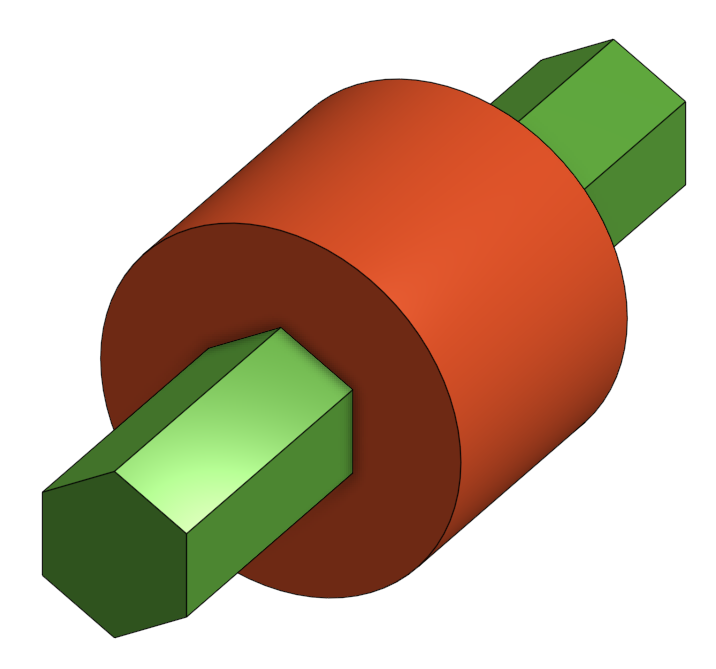
\includegraphics[width=0.6\textwidth]{imgs/hexshaft.png}
			\caption{Hex or other polygon}
		\end{subfigure}
		
		\caption{Shaft-hub geometries.}
	\end{figure}
	\index{shafts!types}
	\index{hubs!types}
	\begin{asparaenum}[a)]
		\item \textit{Keyed}\index{shafts!keyed} shafts, shown in green, have grooves into which \textit{machine keys}\index{machine keys}, shown in blue, can be halfway inserted. The hub, shown in orange, has a groove matching the other half of the key. Set screws, shown in yellow, may be included to clamp down on the key to make sure it doesn't move, and to help secure the key from fretting. These connections are quite common in industrial applications, but their load-carrying capacity is low compared to alternatives.
		\item \textit{D-shafts} have a small flat milled into them. This allows either a hub with a D-shape to mount to it, or a hub that is internally round but has a set screw (yellow) that can tighten down onto the flat. The addition of the flat makes this a much more secure connection than simply tightening the set screw onto a plain round shaft.
		\item \textit{Cross-pins} or bolts can be used to secure shafts. There many variations on this, but one easy to build, easy to maintain, and fairly reliable method is shown. The hub is tapped on one side, and has a hole with clearance for a bolt head on the other side. The shaft has a clearance hole for the bolt. This makes lining up the shafts easy, and the tightening action will help eliminate wobble.
		\item \textit{Splines} are complex geometric shapes with many load-bearing teeth. There are many different standards of splines. These are hard and expensive to produce, but provide the highest torque-transmitting capacity.
		\item \textit{Hex}\index{shafts!hex} and, in general, \textit{polygon}\index{polygon} shafts are a good compromise between cost and load-bearing capacity. Hex is extremely common, especially within the FRC ecosystem and agricultural equipment. Hex stock in many different materials can be readily procured to use as shafting material, and a hex broach can be used to produce the hub.
	\end{asparaenum}
	
\subsection{Bearings, Bushings}
	\index{bearings} \index{bushings}
	Bearings and bushings are components which help eliminate wear between moving surfaces.

	\begin{figure}[H]
		\centering
		\begin{subfigure}[b]{.32\linewidth}
			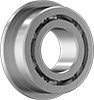
\includegraphics[width=0.7\textwidth]{imgs/ballbearing.png}
			\caption{Ball bearing}
		\end{subfigure}
		\begin{subfigure}[b]{.32\linewidth}
			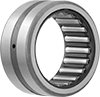
\includegraphics[width=0.7\textwidth]{imgs/needlebearing.png}
			\caption{Needle	 roller bearing}
		\end{subfigure}
		\begin{subfigure}[b]{.32\linewidth}
			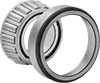
\includegraphics[width=0.7\textwidth]{imgs/tnrbearing.png}
			\caption{Tapered needle roller bearing}
		\end{subfigure}
		\begin{subfigure}[b]{.32\linewidth}
			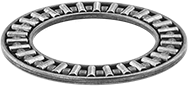
\includegraphics[width=0.7\textwidth]{imgs/thrustbearing.png}
			\caption{Thrust bearing}
		\end{subfigure}
		\begin{subfigure}[b]{.32\linewidth}
			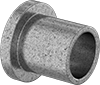
\includegraphics[width=0.7\textwidth]{imgs/plainbushing.png}
			\caption{Plain bushing}
		\end{subfigure}
		
		\caption{Bearings for rotary motion.}
	\end{figure}
	
	\index{bearings!types}
	\begin{asparaenum}[a)]
		\item \textit{Ball bearings} have an inner \textit{race}\index{race} and an outer race with balls in between. These balls are spread out by a cage. They come in many different varieties.
		\begin{asparaitem}[\ \ \ ]
			\item \textit{Sealed} bearings have a rubber seal keeping contaminants out.
			\item \textit{Shielded} bearings have a shield that keeps shrapnel out.
			\item \textit{Open} bearings have no protection whatsoever. Seals and shields trap heat, and necessitate the use of grease rather than oil. This means that in an oily environment (like an engine), open bearings can be much more efficient.
			
			\item \textit{Deep groove} ball bearings are the most common (meaning the balls contact primarily radially).
			\item \textit{Angular contact} and \textit{X-contact} bearings are better at handling thrust and combined loads.
			
			\item \textit{Flanged} bearings have a flange which prevents the bearing from falling through the hole into which they are installed. Not all bearings are flanged.
		\end{asparaitem}
		\item \textit{Needle roller bearings} have an outer race, and inside that, a cage that contains multiple rollers. These bearings can ride directly on a shaft if the shaft is sufficiently hard, or a separate inner race can be used. Needle roller bearings are very low-profile and have very high load-bearing capacities as the rollers distribute load over a larger region. However, they do nothing to retain a shaft axially.
		\item \textit{Tapered needle roller bearings} are heavy-capacity bearings good for combined loading, often used in automotive applications. These mate with a \textit{cup}, much like a needle roller bearing mates with an inner race. These must be used in pairs in opposing directions, and axial preload is necessary for proper operation.
		\item \textit{Thrust bearings} are high-capacity bearings that take thrust (axial) loads rather than radial. This means they are often found in conjunction with needle roller bearings to make a bearing assembly that is high-capacity, compact, and light.
		\item \textit{Plain bushings} are high-capacity, low-RPM single-piece parts. They are made from low-friction materials like oil-impregnated bronze, or plastic. These are good because they are cheap, extremely compact, and very tolerant of improper alignment, dimensional accuracy, and shock loads (since there are no small parts to produce indents).
	\end{asparaenum}
	
	\begin{figure}[H]
		\begin{subfigure}[b]{.32\linewidth}
			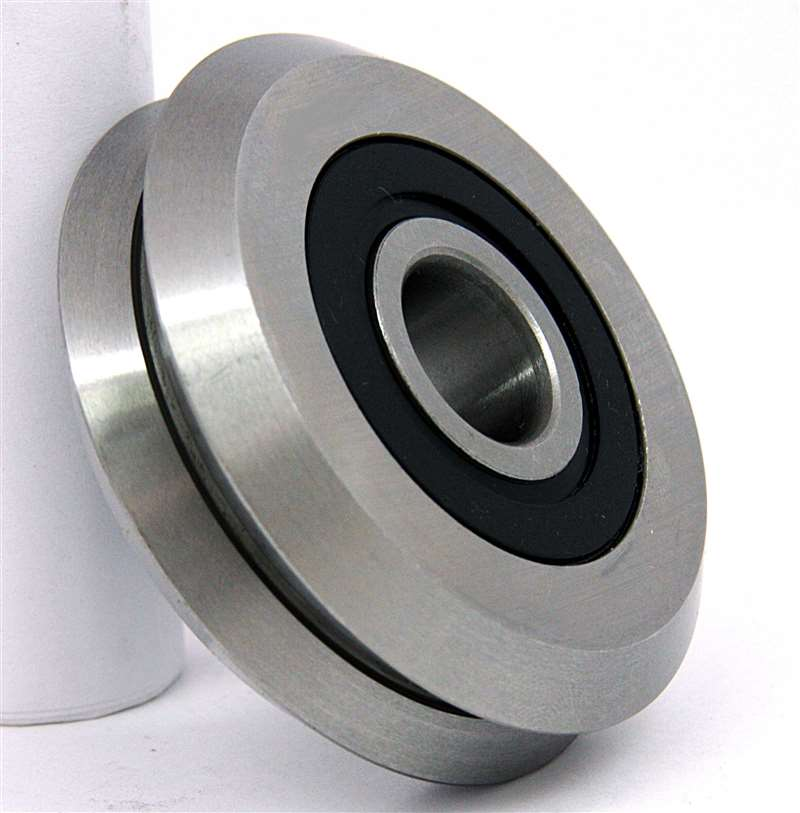
\includegraphics[width=0.7\textwidth]{imgs/vbearing.jpeg}
			\caption{V bearing}
		\end{subfigure}
		\begin{subfigure}[b]{.32\linewidth}
			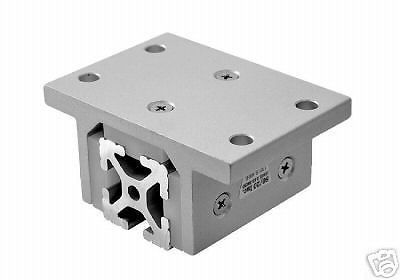
\includegraphics[width=0.7\textwidth]{imgs/8020slider.jpeg}
			\caption{80/20 slider}
		\end{subfigure}
		\begin{subfigure}[b]{.32\linewidth}
			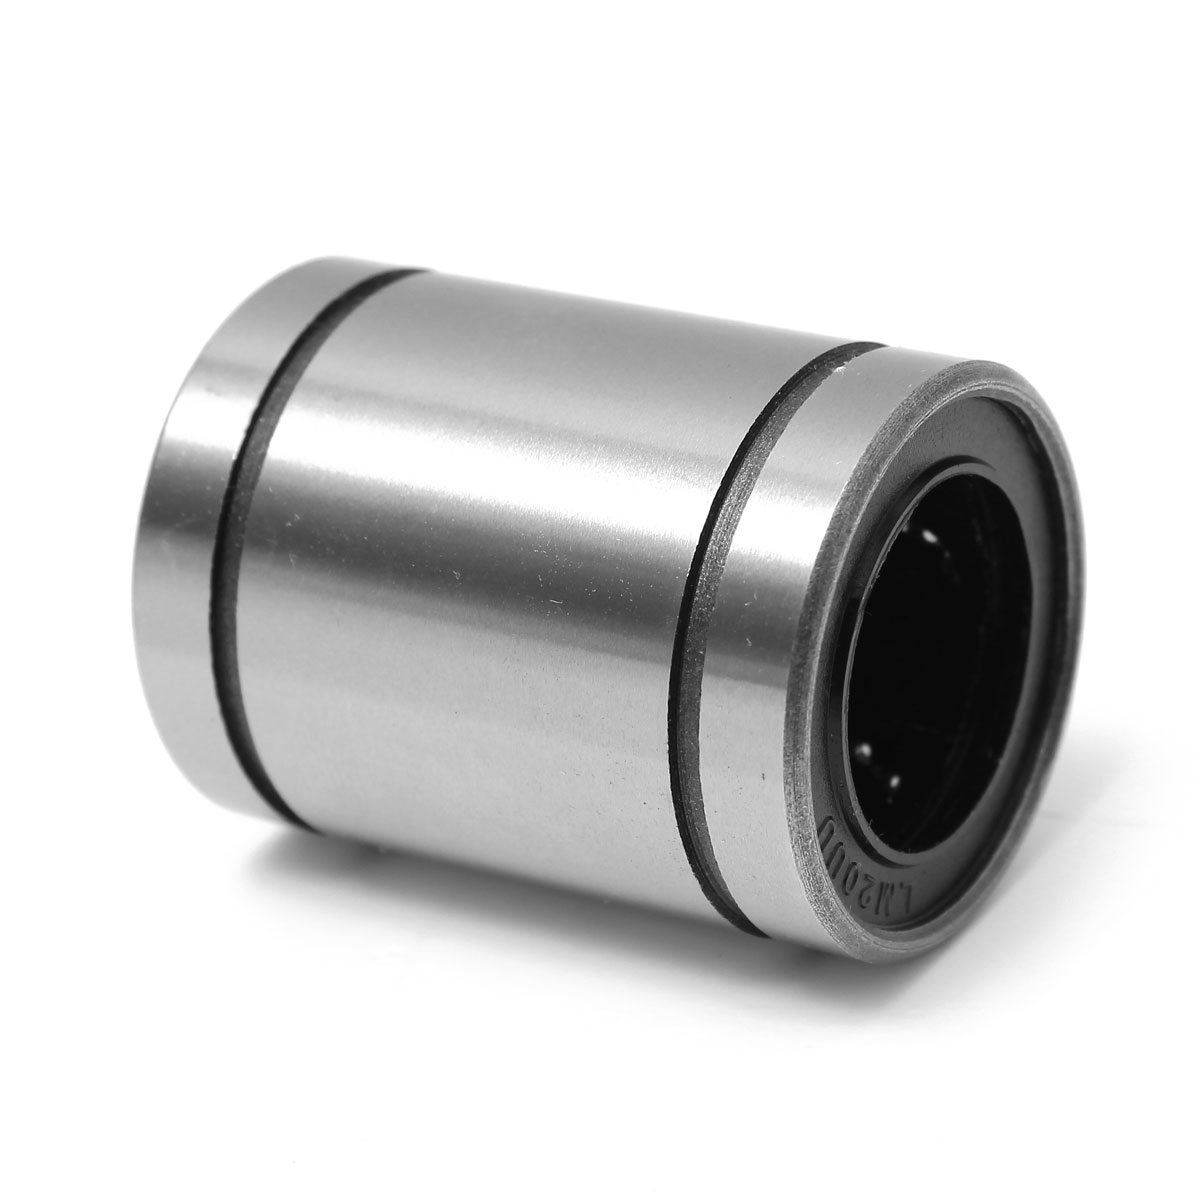
\includegraphics[width=0.7\textwidth]{imgs/linearbearing.jpeg}
			\caption{Linear ball bearing}
		\end{subfigure}
		\begin{subfigure}[b]{.32\linewidth}
			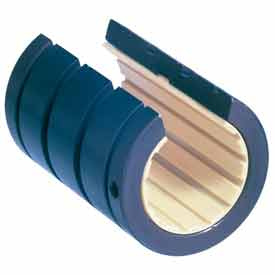
\includegraphics[width=0.7\textwidth]{imgs/linearbushing.jpeg}
			\caption{Linear bushing}
		\end{subfigure}
		\begin{subfigure}[b]{.32\linewidth}
			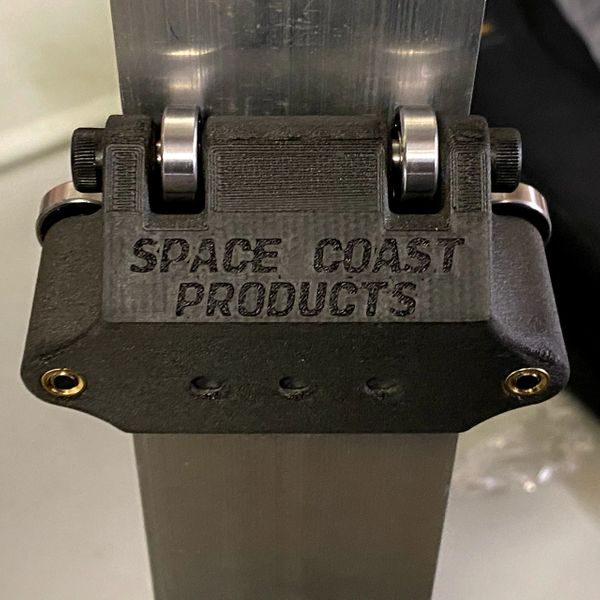
\includegraphics[width=0.7\textwidth]{imgs/elevatorbearingassy.jpeg}
			\caption{Elevator bearing assembly}
		\end{subfigure}
		
		\caption{Bearings for linear motion.}
	\end{figure}
	
	\index{bushings} \index{bearings!linear}
	\begin{asparaenum}[a)]
		\item \textit{V-bearings} can be used in multiples to constrain one part to a rail with appropriate mating geometry.
		\item \textit{Linear sliders} can be used to constrain one part to a rail, cheaply and with a low profile.
		\item \textit{Recirculating linear ball bearings} are high-precision components which are very efficient, which work in conjunction with precision ground rod. These are quite expensive, however, and sensitive to dust, dirt, and shrapnel.
		\item \textit{Linear bushings} are high-precision components which serve the same purpose as linear bearings, but are less sensitive to cleanliness, and often cheaper, although they have higher friction.
		\item \textit{Ball bearings} can be arranged in clever ways on a shaft or tube in order to produce linear guidance.
	\end{asparaenum}

\subsection{Drive Couplings}
	\begin{figure}[H]	
		\begin{subfigure}[b]{.24\linewidth}
			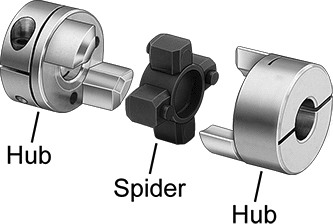
\includegraphics[width=0.7\textwidth]{imgs/coupling_spider.png}
			\caption{Spider coupling}
		\end{subfigure}
		\begin{subfigure}[b]{.24\linewidth}
			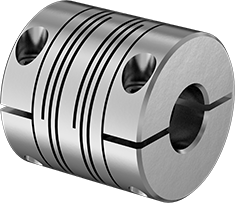
\includegraphics[width=0.7\textwidth]{imgs/coupling_flexible.png}
			\caption{Flexible coupling}
		\end{subfigure}
		\begin{subfigure}[b]{.24\linewidth}
			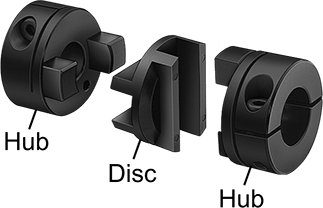
\includegraphics[width=0.7\textwidth]{imgs/coupling_oldham.png}
			\caption{Oldham coupling}
		\end{subfigure}
		\begin{subfigure}[b]{.24\linewidth}
			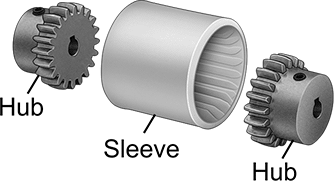
\includegraphics[width=0.7\textwidth]{imgs/coupling_gear.png}
			\caption{Gear coupling}
		\end{subfigure}
		
		\begin{subfigure}[b]{.24\linewidth}
			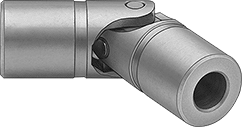
\includegraphics[width=0.7\textwidth]{imgs/coupling_ujoint.png}
			\caption{Universal joint}
		\end{subfigure}
		\begin{subfigure}[b]{.24\linewidth}
			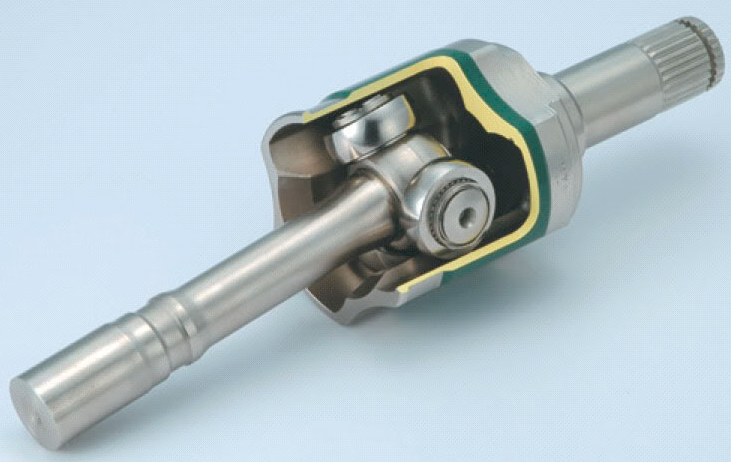
\includegraphics[width=0.95\textwidth]{imgs/coupling_tripod.png}
			\caption{Tripod and tulip}
		\end{subfigure}
		\begin{subfigure}[b]{.24\linewidth}
			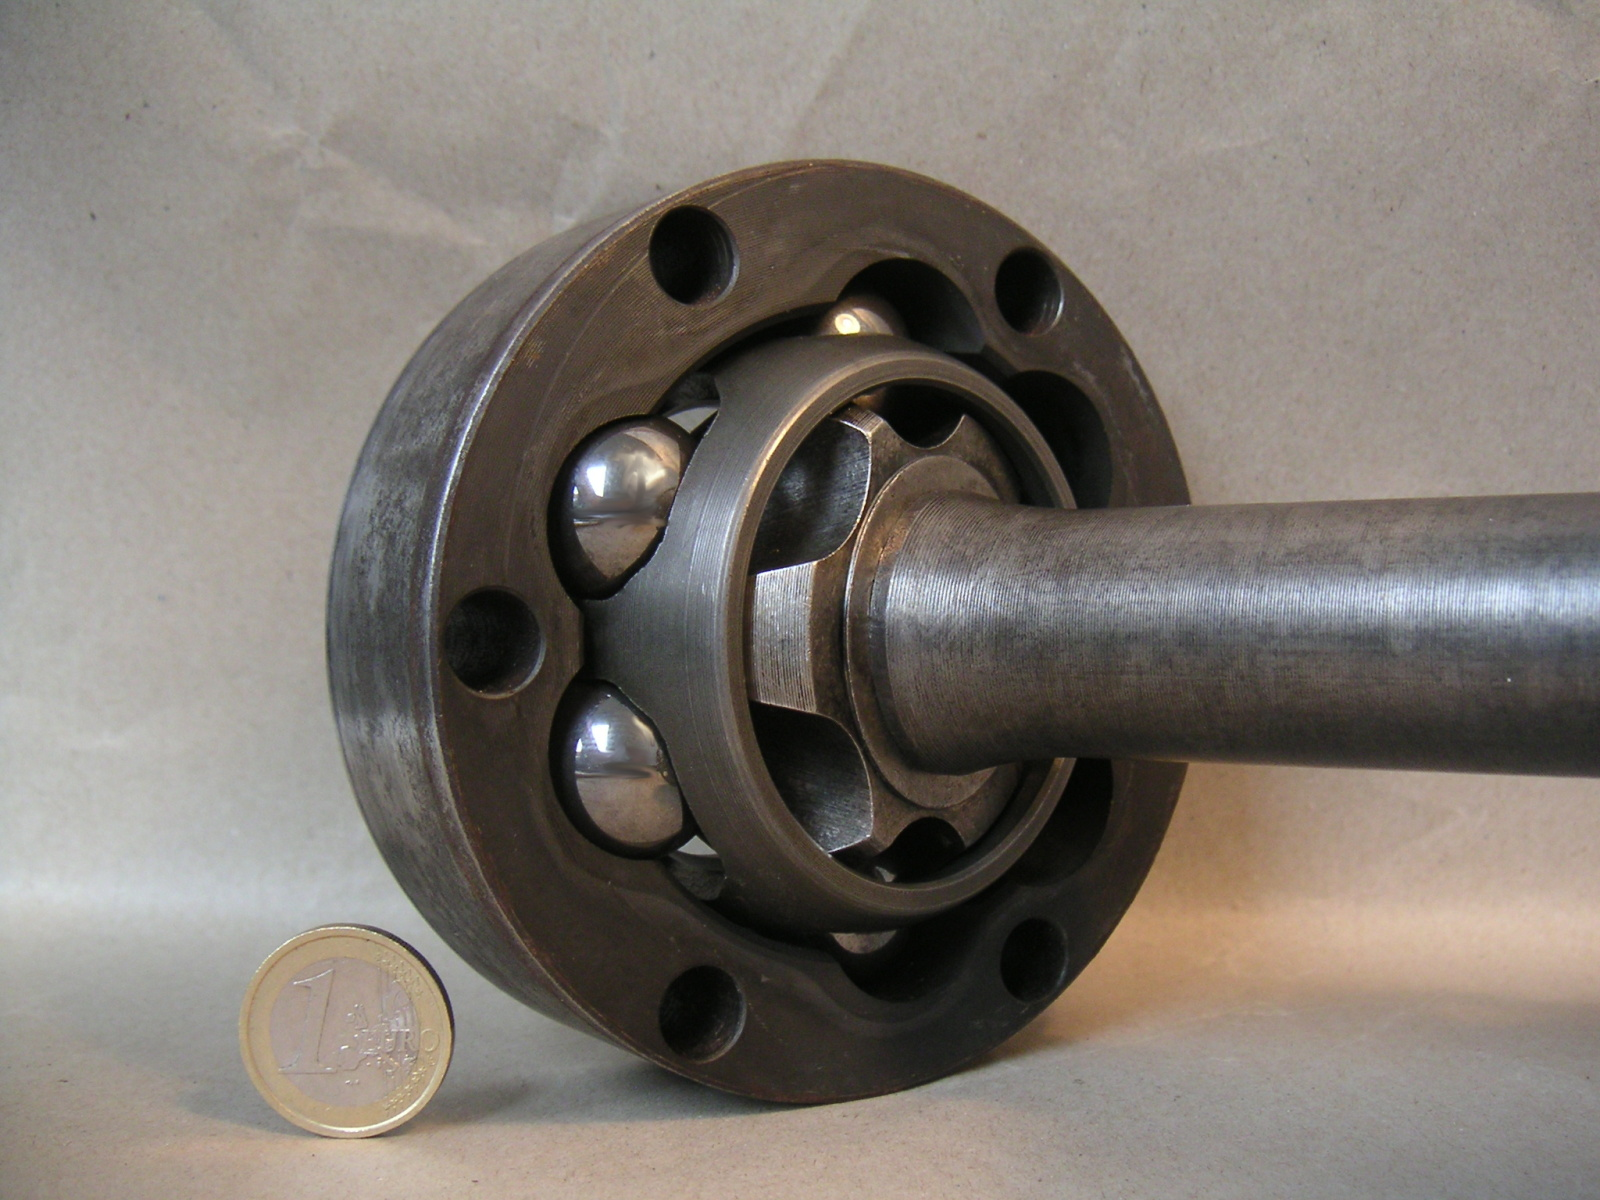
\includegraphics[width=0.85\textwidth]{imgs/coupling_rzeppa.jpeg}
			\caption{Rzeppa joint}
		\end{subfigure}
		\begin{subfigure}[b]{.24\linewidth}
			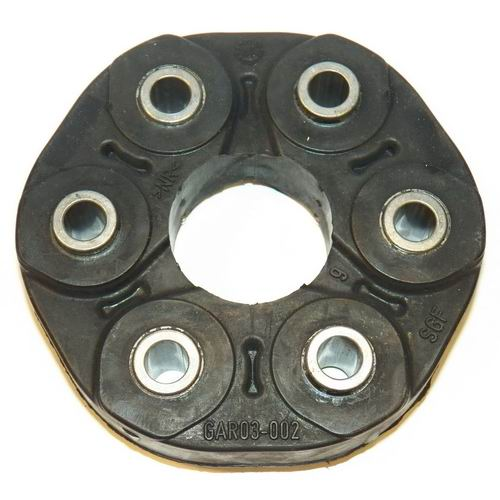
\includegraphics[width=0.7\textwidth]{imgs/coupling_guibo.jpeg}
			\caption{Guibo, or flex disc}
		\end{subfigure}
	\end{figure}

	\index{shaft couplings}
	\begin{asparaenum}[a)]
		\item \textit{Spider couplings} consist of two hubs with teeth that interface with a rubber spider. The rubber spider enables some misalignment of shafts (but does provide some support), and also dampens out vibrations.
		\item \textit{Flexible couplings} are single-body couplings with several slots machined into them in order to make them more flexible. This allows for misalignment of shafts depending on the exact design, while maintaining low backlash.
		\item \textit{Oldham couplings} consist of two hubs with slots that interface with a sliding central portion. They facilitate high shaft misplacement, but do not help with angular or axial misalignment.
		\item \textit{Gear couplings} consist of two spherical hubs with gear teeth cut into them, and a mating sleeve over the hubs. This allows the hubs to plunge inside of the sleeve in addition to being at odd angles, so allows for extreme misalignment, but is quite costly and does present some wear issues at extreme angles.
		\item \textit{Universal joints} or \textit{u-joints} have a central cross-shaped coupling that connects the two u-shaped halves. This enables quite extreme angular misalignment (usually about 30 degrees) However, they are not constant-velocity.
		\item \textit{Tripods} are a type of \textit{constant-velocity (CV) joint}\index{shaft couplings!constant-velocity}. These consist of three bearings fixed to a hub. The bearings contact a tulip and slide back and forth on it. This joint can handle decent angular misalignment (usually about 15 degrees) and allows for axial movement, referred to as \textit{plunging}.
		\item \textit{Rzeppa joints} are another CV joint. These joints cannot plunge, but do allow for severe angular misalignment (usually about 45 degrees). Front-wheel drive cars often use shafts where the differential side has a tripod joint and the wheel side has a rzeppa joint. This way the shaft can plunge, and the wheel can be powered and steered.
		\item \textit{Guibos} or \textit{flex discs} are a joint (can can be considered a CV joint) which use two hubs connected by some flexible (usually rubber) coupling. This helps to absorb vibrations, and handles shaft misalignment.
	\end{asparaenum}

	\begin{mdframed}[style=QuestionBox]
		What is this "constant velocity" behavior, and why is it important in some applications?
	\end{mdframed}

\section{Nonaxial Power Transmission}

We often need to transmit power from one place to another not in a line. We also often need to change the torque and speed ratios of the power. There are many ways of doing this.

\subsection{Rope and Pulleys}
\index{rope}
\index{pulleys}
Ropes, pulleys, and spools are the simplest way to transmit power from one place to another. They aren't particularly technical, but there are a few nuances which can be used to help design systems using them.

\begin{figure}[H]	
	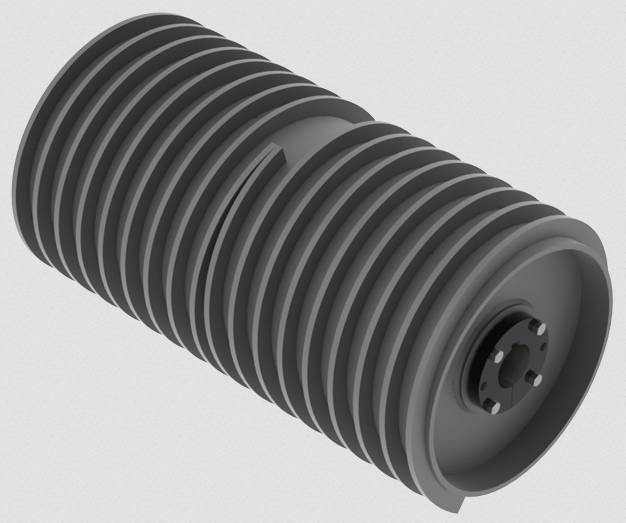
\includegraphics[width=0.4\textwidth]{imgs/takeup_pulley.png}
	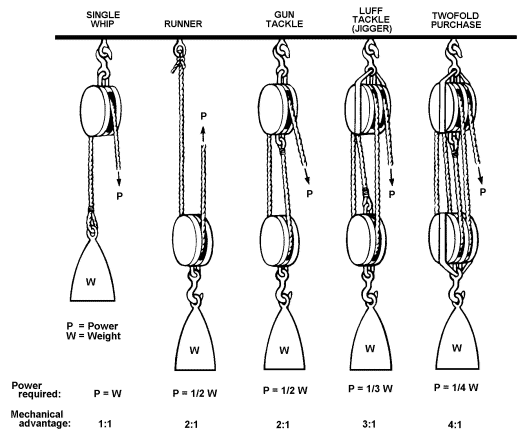
\includegraphics[width=0.5\textwidth]{imgs/block_tackle.png}
	\caption{Left: helical takeup pulley. Right: various block and tackle.}
\end{figure}

Helical takeup pulleys have grooves in them which help route rope so that when it is wound, it is wound at a constant radius. This can help prevent binding or slack in closed-loop systems (like continuous rigging elevators). To help closed loop systems more, a spring inline with the rope can take up more slack than a stiff rope. \href{https://youtu.be/kyfb8lGAveY?t=5}{\color{red}\underline{Video Example (0:05)}}

A \textit{block and tackle}\index{pulleys!block and tackle} is a system of two or more pulleys with a rope routed between them in alternating fashion as shown. This generates mechanical advantage; the rope must be pulled more to achieve the same lifting force. This also decreases the input load required to raise the load by a factor of the number of ropes. 

\subsection{Gears}

A \textit{gear}\index{gear} is effectively, a wheel with teeth. These teeth are specially shaped in order to \textit{mesh} and mate nicely with other gears, so you need to be careful that you're using gears that are compatible with each other, and spacing them far enough apart.

\begin{figure}[H]
	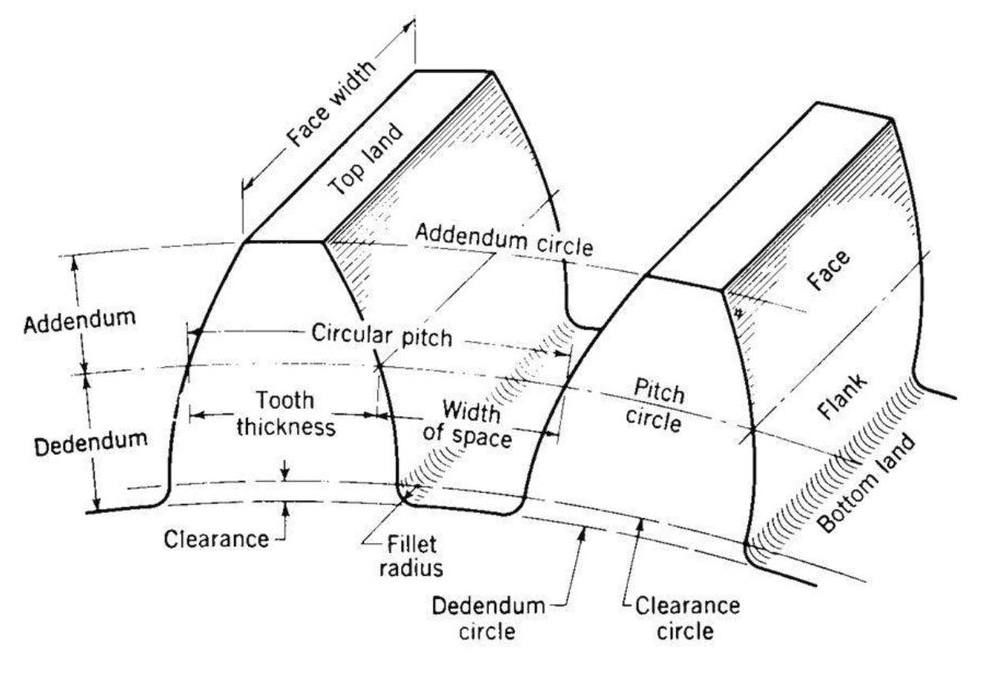
\includegraphics[width=0.8\textwidth]{imgs/gear_nomenclature.png}
	\caption{Nomenclature of different gear dimensions}
\end{figure}
\index{gear!nomenclature}
Gears are specified, among other things, by the number of teeth, their \textit{pressure angle}\index{gear!pressure angle}, and either the \textit{diametral pitch}\index{gear!diametral pitch} or \textit{module}\index{gear!module}.

\begin{asparaenum}[a)]
	\item Gear teeth have an \textit{involute} profile. This is a specific geometric shape that is not quite an arc, but makes sure power transmission is smooth; without excessive backlash.
	\item The \textit{pitch circle} is a rough representation of the gear as a wheel. It lies somewhere in between the overall diameter and the diameter of the root of the teeth. You can draw up a sketch containing gears' pitch circles tangent to each other, and then they will fit together.
	\item A gear's \textit{diametral pitch} (DP) is the number of teeth in a gear divided by the pitch diameter (in inches). So, if a gear has 50 teeth and is a 20DP gear, it would have a pitch circle of diameter $50 \ teeth \ / \ 20 \ DP = 2.5 \ inches$. For two gears to be compatible and mesh, they must have the same diametral pitch, otherwise the teeth would be the wrong sizes.
	\item A gear's \textit{module} is a gear's pitch diameter (in mm) divided by the number of teeth. This measures the same thing as diametral pitch, just in a different way. If a 5 module gear has 30 teeth, its pitch diameter would be $5 \ mm \times 30 \ teeth = 150 \ mm$.
	\item A gear's \textit{pressure angle}(PA) measures how steep the teeth are, or the angle of the contact line. This must be the same between two gears for them to be compatible. There is a lot of testing and science behind picking a good angle; higher angles are weaker and produce higher loads on the system, but do make oil flow better. Usually, though, this isn't a big concern- just make sure that you don't mix and match pressure angles. 14.5 degrees is common for greased gears.
\end{asparaenum}

\index{gear!types}
\begin{figure}[H]
	\begin{subfigure}[b]{.32\linewidth}
		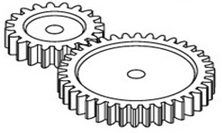
\includegraphics[width=0.8\textwidth]{imgs/gear_spur.png}
		\caption{Spur}
	\end{subfigure}\begin{subfigure}[b]{.32\linewidth}
		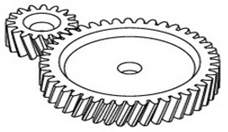
\includegraphics[width=0.8\textwidth]{imgs/gear_helical.png}
		\caption{Helical}
	\end{subfigure}\begin{subfigure}[b]{.32\linewidth}
		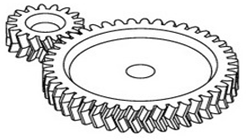
\includegraphics[width=0.8\textwidth]{imgs/gear_herringbore.png}
		\caption{Herringbone}
	\end{subfigure}
	
	\begin{subfigure}[b]{.32\linewidth}
		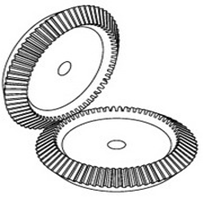
\includegraphics[width=0.8\textwidth]{imgs/gear_bevel.png}
		\caption{Bevel}
	\end{subfigure}\begin{subfigure}[b]{.32\linewidth}
		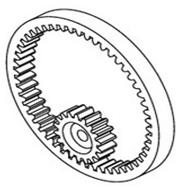
\includegraphics[width=0.8\textwidth]{imgs/gear_ring.png}
		\caption{Ring}
	\end{subfigure}\begin{subfigure}[b]{.32\linewidth}
		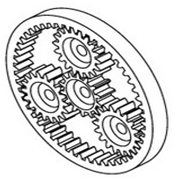
\includegraphics[width=0.8\textwidth]{imgs/gear_planetary.png}
		\caption{Planetary set}
	\end{subfigure}
	
	\begin{subfigure}[b]{.32\linewidth}
		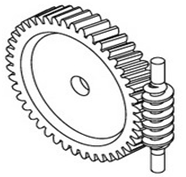
\includegraphics[width=0.8\textwidth]{imgs/gear_worm.png}
		\caption{Worm}
	\end{subfigure}\begin{subfigure}[b]{.32\linewidth}
		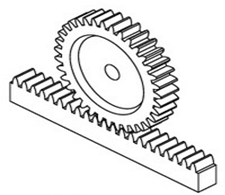
\includegraphics[width=0.8\textwidth]{imgs/gear_rack_pinion.png}
		\caption{Rack \& pinion}
	\end{subfigure}
	\caption{Various different gear sets.}
\end{figure}

\begin{asparaenum}[a)]
	\item \textit{Spur} gears have straight-cut teeth. This means they are two-dimensional and relatively simple to produce.
	\item \textit{Helical} gears have angled-cut teeth. These are harder to produce, but they create smoother power transmission since multiple teeth are in contact, creating a seamless hand off. However, the helical nature produces an axial load in addition to the radial load that gears already produce. 
	\item \textit{Herringbore} gears are effectively two helical gears back-to-back. This causes the axial loads that helical gears produce to cancel out. This type of gear, though, is obviously even more complicated to produce.
	\item \textit{Bevel}\index{gear!bevel, miter} gears allow power transmission along non-parallel axes. It is important to note that bevel gears are made as sets- you cannot use a 40T gear intended for use with a 20T, with a 60T, as the angles will not mesh up.
	\item \textit{Ring} gears are simply inverse spur gears.
	\item \textit{Planetary}\index{gear!planetary} gear sets are compact reductions that can be configured in many ways depending on which part of the set is fixed in place. Typically, the ring is held fixed, the central \textit{sun gear} is driven, and a \textit{carrier plate} (now shown) holding the \textit{planet gears} is the output.
	\item \textit{Worm} gears are extremely compact reductions, but are often not very efficient. The worm wheel (right) might have one or several \textit{leads}, or teeth. A lower number of leads will reduce the gear set's ability to be backdriven, which can be a desirable characteristic.
	\item A \textit{rack and pinion}\index{gear!rack and pinion} can be used to transform rotary motion into linear motion, or vice versa.	
\end{asparaenum}

A \textit{gearbox} which contains multiple gears constrained with bearings must be designed to withstand the various loads produced by gears.

\begin{figure}[H]
	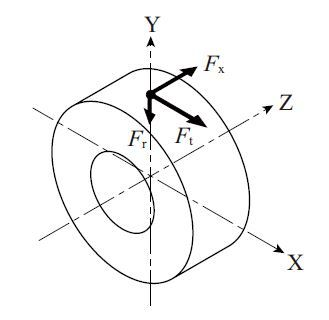
\includegraphics[width=0.5\textwidth]{imgs/gear_forces.jpeg}
	\caption{Forces on a gear tooth.}
\end{figure}

\begin{asparaenum}[a)]
	\item \textit{Tangential force} is found simply as $F_{t} = T_{gear} / r_{pitch, gear}$, and is the major and obvious load that must be withstood.
	\item \textit{Radial force} is produced as a result of the pressure angle. It can be computed as $F_{r} = F_{t} \text{tan}(\alpha)$ where $\alpha$ is the pressure angle. As such, higher pressure angles will produce higher radial forces, which will push gears apart.
	\item \textit{Thrust force} exists for helical gears and is computed as $F_{x} = F_{t} \text{tan}(\beta)$ where $\beta$ is the helix angle.
\end{asparaenum}

\begin{figure}[H]
	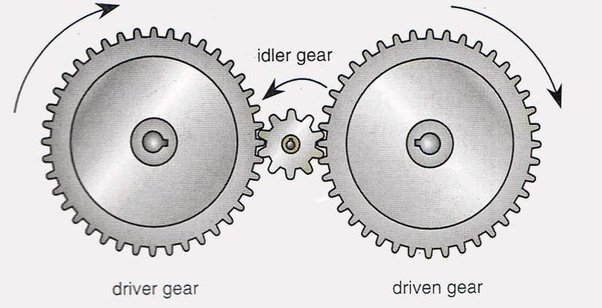
\includegraphics[width=0.6\textwidth]{imgs/gearset_idler.jpeg}
	\caption{A spur gear set with a idler gear (middle).}
\end{figure}

\index{gear!idler}
\textit{Idlers} can be introduced to a gear set to change the direction of rotation, or to bridge a large gap and transmit power from one place to another. The idler does not impact the overall gear ratio, only the direction of motion.

\index{differential}
\textit{Differentials} are a special arrangement of gears that can be used to produce differential motion
\begin{align}
	\omega_{input} = \frac{\omega_{left} + \omega_{right}}{2} .
\end{align}

This is desirable as a speed difference can be had between the left and right sides (for instance, a car that is turning has its wheels running at different speeds) while still sending power to both.

\begin{figure}[H]
	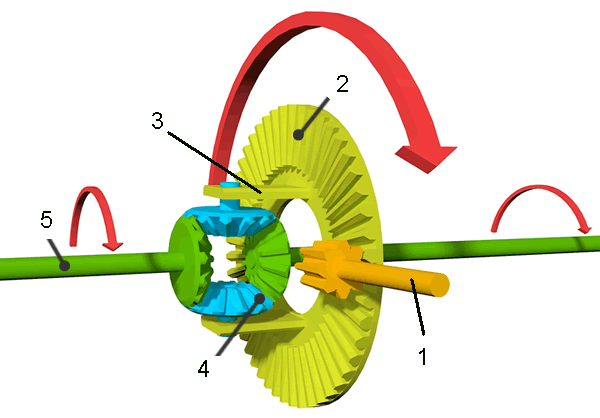
\includegraphics[width=0.8\textwidth]{imgs/differential.png}
	\caption{A differential.}
\end{figure}

A plain or \textit{open} differential uses an outer casing to drive a central \textit{spider} gear. This spider is connected to the left and right gears. Analysing the torque balance on the spider gear reveals

\begin{align}
	\Sigma T &= m \alpha = 0 \nonumber \\
	0 &= \frac{T_{left}}{r_{left}} r_{spider} - \frac{T_{right}}{r_{right}} r_{spider}  \nonumber \\
	T_{left} &= T_{right} \text{ if } r_{left} = r_{right}
\end{align}

Analysing the torque balance on the whole differential reveals

\begin{align}
	\Sigma T &= m \alpha = 0 \nonumber \\
	0 &= T_{left} + T_{right} - T_{input} \nonumber \\
	T_{left} = T_{right} &= \frac{T_{input}}{2}
\end{align}

As such, the open differential makes the torque on each wheel the same. This can be problematic if one wheel loses traction, as the other wheel will have its torque capacity correspondingly reduced. \index{differential!limited-slip} \textit{Limited-slip} differentials employ additional components or techniques such as clutch packs to limit the amount of speed difference $|\omega_{left} - \omega_{right}|$ and/or the amount of torque difference $|T_{left} - T_{right}|$ to continue delivering power in adverse conditions. 

\begin{mdframed}[style=QuestionBox]
	An adder-subtractor is an arrangment of differentials and gears that can be quite useful. Why would you want to use something like it? (Look up: ``differential swerve", ``differential elevator", ``adder-subtractor module").
\end{mdframed}	

\newpage

\subsection{Roller Chain and Sprockets}

\textit{Roller chain}\index{chain} is a robust way of transmitting power from one place to another. 

\begin{figure}[H]
	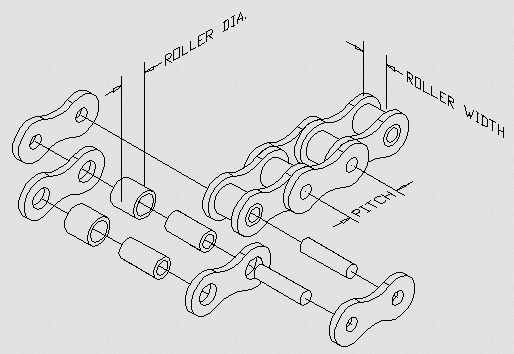
\includegraphics[width=0.7\textwidth]{imgs/rollerchain_nomenclature.png}
	\caption{Roller chain exploded view, and dimensions}
\end{figure}

Chain is dimensioned by the \textit{roller diameter}, \textit{roller width}, and \textit{chain pitch}, but may have a standard number that details all of these. Table \ref{table:chaindims} lists some common sizes.

\begin{table}[H] 
\begin{tabular}{llll}
Chain \# & Pitch (in) & Roller Width (in) & Roller Diameter (in) \\
25       & 0.250      & .125              & .130                 \\
35       & 0.375      & .188              & .200                 \\
40       & 0.500      & .312              & .312                 \\
41       & 0.500      & .250              & .306                
\end{tabular}
\caption{Common roller chain dimensions.}
\label{table:chaindims}
\end{table}
\index{chain!dimensioning}

\begin{figure}[H]
	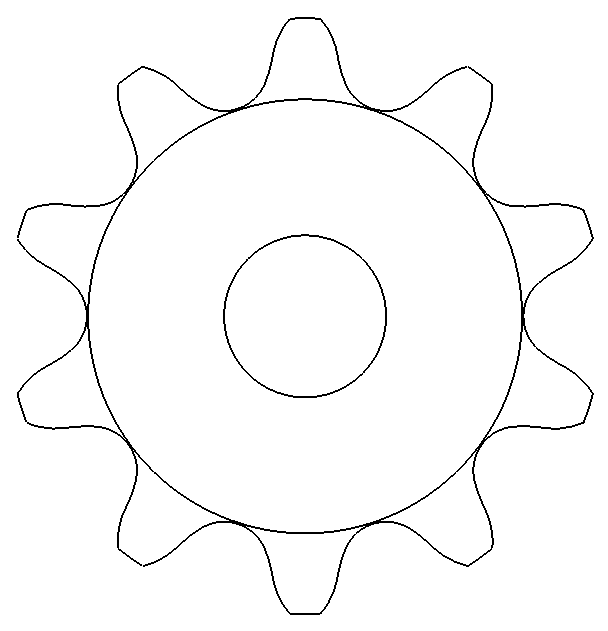
\includegraphics[width=0.3\textwidth]{imgs/sprocket_profile.png}
	\caption{A sprocket's profile.}
\end{figure}

\textit{Sprockets}\index{chain!sprockets} are shaped specially to mesh with chain- they are not gears. \textit{Hub} sprockets are designed to mount directly to a shaft, while \textit{plate} sprockets mount with a bolt pattern to another mechanism, or a hub.

\begin{figure}[H]
	\begin{subfigure}[b]{.32\linewidth}
		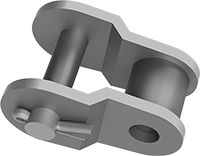
\includegraphics[width=0.8\textwidth]{imgs/chain_halflink.png}
		\caption{Half link}
	\end{subfigure}\begin{subfigure}[b]{.32\linewidth}
		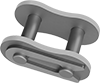
\includegraphics[width=0.8\textwidth]{imgs/chain_masterlink.png}
		\caption{Master link}
	\end{subfigure}\begin{subfigure}[b]{.32\linewidth}
		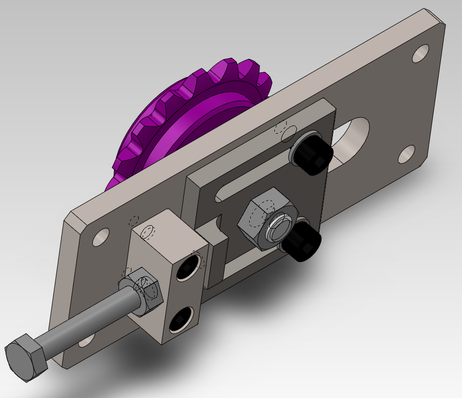
\includegraphics[width=0.8\textwidth]{imgs/chain_axletens.png}
		\caption{Axle position adjustment}
	\end{subfigure}
	
	\begin{subfigure}[b]{.32\linewidth}
		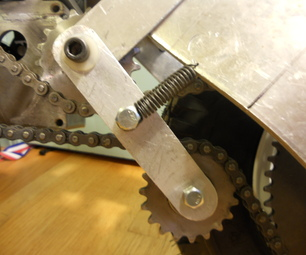
\includegraphics[width=0.8\textwidth]{imgs/chain_idler.jpeg}
		\caption{Idler sprocket}
	\end{subfigure}\begin{subfigure}[b]{.32\linewidth}
		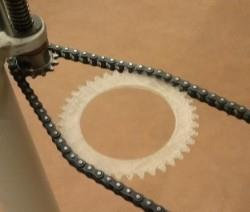
\includegraphics[width=0.8\textwidth]{imgs/chain_floater.jpeg}
		\caption{Floater}
	\end{subfigure}\begin{subfigure}[b]{.32\linewidth}
		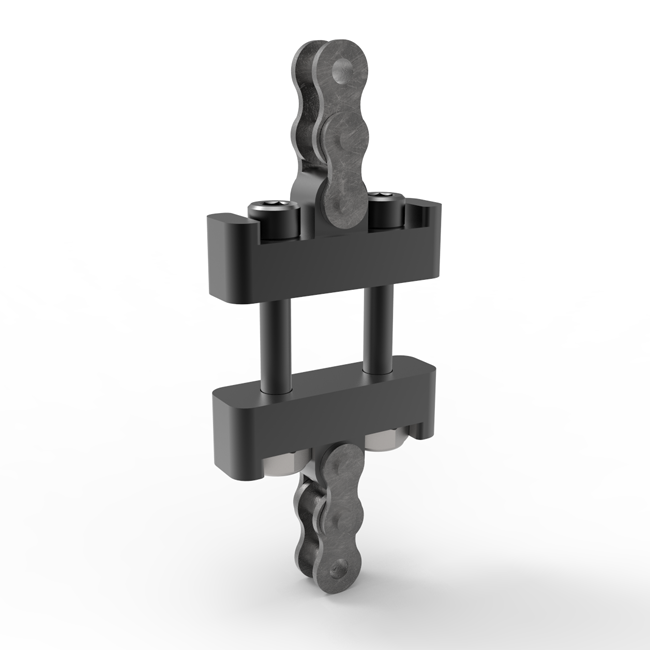
\includegraphics[width=0.8\textwidth]{imgs/chain_inlinetens.png}
		\caption{Inline tensioner}
	\end{subfigure}
	
	\caption{Various different adjustment methods for chain.}
\end{figure}

Chains need to be properly tensioned to make sure that they do not skip, to reduce the backlash of the system, and still run smoothly. If they are too tight, they can bind. If too lose they can skip teeth and throw the chain off the sprockets.

\index{chain!adjustment, tensioning}
\begin{asparaenum}[a)]
	\item \textit{Half links} can be used for coarse adjustment. Normally roller chain is made of connecting links and outer pin links, so adjustments can only be done in lengths of $2 \ \times \ pitch$, but half links allow adjustments of exactly the pitch. However, these half-links are often significantly weaker than 
	\item \textit{Master links} are quickly removable links of a chain that use a clip to retain the pins rather than being pressed into position. This clip has a nonzero chance of falling off.
	\item \textit{Moving the distance of the axles} is an easy method of adjusting the tension. This can be accomplished in a multitude of ways. This may not be easy to accomplish, however.
	\item \textit{Idler} rollers or tensioners may be added to increase the tension by re-routing the chain. They may be spring-loaded or automatic, or fixed. These (sometimes in multiples) can also be used to increase chain wrap.
	\item \textit{Floating sprockets} can be added to increase the tension. These can be further adjusted by moving the floater away from the center and towards the ends.
	\item \textit{Inline tensioners} can be used when the chain does not make full revolutions. These are easy to integrate and are very low-profile.
\end{asparaenum}

\begin{figure}[H]
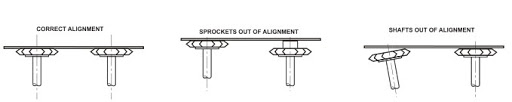
\includegraphics[width=0.9\textwidth]{imgs/chain_alignment.jpeg}
\caption{Sprocket alignment.}
\end{figure}
\index{chain!alignment}

Sprockets and the axles they ride on must be aligned properly otherwise there is a risk of throwing the chain.

Wrap is another important consideration for chain drives. If there is not enough teeth in engagement with the sprocket, the sprocket may wear out or break, or the chain may skip. 

\newpage
\subsection{Belts, Pulleys}

\begin{figure}[H]
	\begin{subfigure}[b]{.24\linewidth}
		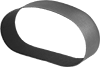
\includegraphics[width=0.8\textwidth]{imgs/belt_flat.png}
		\caption{Flat belt}
	\end{subfigure}\begin{subfigure}[b]{.24\linewidth}
		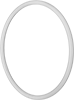
\includegraphics[width=0.6\textwidth]{imgs/belt_round.png}
		\caption{Polycord / round belt}
	\end{subfigure}\begin{subfigure}[b]{.24\linewidth}
		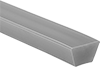
\includegraphics[width=0.9\textwidth]{imgs/belt_v.png}
		\caption{V belt}
	\end{subfigure}\begin{subfigure}[b]{.24\linewidth}
		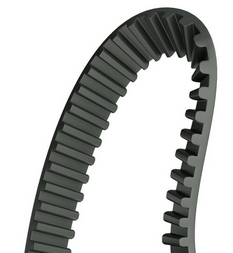
\includegraphics[width=0.65\textwidth]{imgs/belt_timing.png}
		\caption{Timing belt}
	\end{subfigure}
	\caption{Various drive belts.}
\end{figure}

A \textit{belt}\index{belts} is a continuous loop of a flexible material. There are many different types of belts.

\begin{asparaenum}[a)]
	\item \textit{Flat belts}\index{belts!flat} are flat in cross-section with no special features. They transmit power solely by friction. A crowned pulley, proper tensioning (about 1-3\% stretch for polyurethane belts), and alignment keeps the belt from walking side-to-side excessively.
	\begin{figure}[H]
		\includegraphics[width=0.6\textwidth]{imgs/belt_crown_pulley.jpeg}
		\caption{Crowning on pulleys to keep flat belts on pulleys.}
	\end{figure}
	\item \textit{Polycord} or \textit{round belt}\index{belts!round} is round in cross-section. They are somewhat forgiving in how much they can be tensioned (as long as ample stretch is provided; around 10\% for polyurethane cords). They work best with pulleys that have a 60 degree (included angle) V cut into them.
	\item \textit{V-belts}\index{belts!V-belts} have a V cross-section that digs in to pulleys. Multiple vees may be attached side-by-side for increased flexibility. They (usually) have reinforcing fibers that provide strength and stiffness much higher than pure rubber. Sometimes they have teeth in them, but these teeth are not for power transmission, they are simply to allow greater flexibility in the belt while still allowing for a tall, centering profile.
	\item \textit{Timing belt}\index{belts!timing} has teeth to ensure positive transmission of motion (so it can be used to time multiple components together). It has very high load-carrying potential without need for perfect tensioning. Like v-belts, they have reinforcing fibers that provide strength and stiffness much higher than pure rubber. There are many different series of timing belts (HTD, GT2, MXL, etc.) - they are not compatible with each other. In FRC the most common are HTD and GT2 (which are, actually, semi-compatible). The pitches must also be the same in addition to the series.
\end{asparaenum}

Belts, like chain, must be properly tensioned and aligned. Most of the methods explained for chains also work for belts. Special considerations must be made for the back-bending capacity of the belt in question (every belt has a rated back-bending radius). Pulleys for timing belts usually require at least six (6) teeth of engagement, although this may increase or decrease based on your load case and manufacturer's recommendations.  Timing belt doesn't need tensioning, just correct and precise spacing.

My \href{http://thaddeus-maximus.github.io/swissarmyengineer/}{\color{red}\underline{EveryCalc}} has a calculator to determine the length of belt needed to achieve a certain center-to-center distance (or vice versa) for flat belts, polycord, and timing belts.

\begin{figure}[H]
	\includegraphics[width=0.5\textwidth]{imgs/belt_crossed.png}
	\caption{Crossed drive belt}
\end{figure}
	Belts can be crossed in order to transmit power while reversing direction, or even transmit power between non-parallel axles. This generally works best with polycord, but can be accomplished with any belt.
	
\section{Lead Screws}
\begin{figure}[H]
	\includegraphics[width=0.5\textwidth]{imgs/lead_screw.png}
	\caption{Lead screw and nut}
\end{figure}

\textit{Lead screws} are specially-formed screws that are intended for power transmission. They are used in conjunction with a correspondingly threaded nut to transform rotational motion into linear motion. Like worm gears, they may have multiple \textit{leads}, and depending on the angle, may be self-locking. The more leads and the coarser the thread pitch, the slower the nut will move, the efficiency will be decreased, and the arrangement will be more self-locking.

\begin{figure}[H]
	\includegraphics[width=0.5\textwidth]{imgs/thread_forms.png}
	\caption{Different thread forms}
\end{figure}

While typical screws use triangular thread forms, there are more types for lead screws, and lead screws generally have a much higher surface finish since they will be screwed and unscrewed repeatedly.
\begin{asparaenum}[a)]
\item \textit{Square} threads offer superior performance and reduced sliding friction. However, they are much harder to produce.
\item \textit{Acme} threads are a particular standard using trapezoidal-shaped threads. The increased size of the thread provides more strength, and they have a shallower angle than a typical thread, providing a compromise from a square thread for manufacturability sake.
\item \textit{Buttress} threads are asymmetrical, intended to be loaded dominantly in one direction (e.g. for a lift).
\item \textit{Ball screws} have round cutouts intended for recirculating ball carriers. These are a class of their own, requiring the highest precision, but offerring the most efficient power transfer.
\end{asparaenum}
	
\section{Energy Storage} \label{sec:energy_storage}

\subsection{Springs} \label{subsec:springs} \index{spring}
	Springs are components designed explicitly to change shape by a great distance and store energy in the process.
	
	\begin{figure}[H]
		\begin{subfigure}[b]{.19\linewidth}
			\includegraphics[width=0.9\textwidth]{imgs/spring_extension.png}
			\caption{Extension}
		\end{subfigure}\begin{subfigure}[b]{.19\linewidth}
			\includegraphics[width=0.9\textwidth]{imgs/spring_compression.png}
			\caption{Compression}
		\end{subfigure}\begin{subfigure}[b]{.19\linewidth}
			\includegraphics[width=0.9\textwidth]{imgs/spring_torsion.png}
			\caption{Torsion}
		\end{subfigure}\begin{subfigure}[b]{.19\linewidth}
			\includegraphics[width=0.4\textwidth, angle=-90]{imgs/spring_progressive.png}
			\caption{Progressive}
		\end{subfigure}
		
		\begin{subfigure}[b]{.19\linewidth}
			\includegraphics[width=0.9\textwidth]{imgs/spring_leaf.png}
			\caption{Leaf}
		\end{subfigure}\begin{subfigure}[b]{.19\linewidth}
			\includegraphics[width=0.6\textwidth, angle=90]{imgs/spring_conforce.png}
			\caption{Constant-force}
		\end{subfigure}\begin{subfigure}[b]{.19\linewidth}
			\includegraphics[width=0.6\textwidth]{imgs/spring_rotor.png}
			\caption{Rotor}
		\end{subfigure}\begin{subfigure}[b]{.19\linewidth}
			\includegraphics[width=0.8\textwidth]{imgs/spring_elastic.png}
			\caption{Surgical tubing}
		\end{subfigure}\begin{subfigure}[b]{.19\linewidth}
			\includegraphics[width=0.9\textwidth]{imgs/spring_gasshock.png}
			\caption{Gas shock}
		\end{subfigure}
	\end{figure}
	
	\begin{asparaenum}[a)]
		\item \textit{Extension} \index{spring!extension} springs can be pulled on to provide tension. They have hooks or loops on either end for attachment. They provide force $F$ proportional to the distance $\Delta x$ they have been stretched from their relaxed state.
		\begin{align}
			F_{spring} = k \Delta x
		\end{align}
		\item \textit{Compression} \index{spring!compression} springs can be pushed on to provide compressive resistance. There are different styles of ends (open, closed, closed and ground). Like extension springs they have a linear force ratio.
		\item \textit{Torsion} \index{spring!torsion} springs can be bent to provide resistance. They come in different windings and are designed to be bent in a particular way and not the other. Like extension springs they have a linear force ratio (although the units may be angular).
		\item \textit{Progressive} \index{spring!compression!progressive} springs are compression springs that have variable windings. As they are compressed, the tighter wound windings bottom out, increasing the spring rate $k$.
		\begin{align}
			F_{spring,\ progressive} = k(\Delta x) \Delta x \ \mbox{where} \ \frac{d k(\Delta x)}{d \Delta x} > 0
		\end{align}
		\item \textit{Leaf} \index{spring!leaf} springs are flat strips, sometimes stacked on top of each other. Commonly used in truck suspensions as they can also act as suspension links in their stiff direction.
		\item \textit{Constant force springs} \index{spring!constant-force} are thin strips of stainless steel that are tightly coiled. The strip can be secured to one object while the rest of the coil is secured to another object. Unlike other springs, the force does not vary much with distance, making them ideal for many scenarios.
		\begin{align}
			F_{spring, \ constant-force} \approx F_k
		\end{align}
		\item \textit{Rotor} \index{spring!rotor} springs can be wound many times to provide not quite constant, but close to constant force as the coils unwind.		
		\item \textit{Elastic} \index{spring!elastic} such as \textit{surgical tubing} can be used as a cheap and adjustable source of springiness. Surgical tubing can be easily mounted with zip ties and the insertion of a plug into the ends.
		\item \textit{Gas shocks} provide not only spring force, but damping as air is throttled through a small orifice. They also come as bolt-on units, making packaging quite clean.
	\end{asparaenum}
	
	\subsection{Flywheels}
	\index{flywheel}
	\begin{figure}[H]
		\includegraphics[width=0.6\textwidth]{imgs/flywheel.jpeg}
		\caption{A flywheel.}
	\end{figure}
	\textit{Flywheels} are discs of material which are intended to spin at high speed to store energy for future use. This could be to even out the vibrations in an engine, or to store energy in a flywheel-based shooter. They are specified by their \textit{moment of inertia} $I$. \index{moment of inertia}
	
	This moment of inertia can be computed with a volume integral:
	\begin{align}
		I = \int_{\volume} \rho r^2 d \volume ,
	\end{align}
	
	where $\rho$ is the density of the material and $r$ is the distance from the axis of rotation. This may be confusing and not mean but much to you, but the takeaway is this: a larger (bigger $r$), denser (bigger $\rho$) flywheel has a higher moment of inertia, so can store more energy. By placing the mass of a flywheel far away from the center and hollowing out the center, the moment of inertia can be increased while minimizing mass.	
	
	
\section{Wheels} \label{sec:wheels} \index{wheel}
	There are many different types of wheels so they're worth of their own section.
	
	\subsection{Hard Wheels}
	
	\begin{figure}[H]
		\begin{subfigure}[b]{.24\linewidth}
			\includegraphics[width=0.9\textwidth]{imgs/wheel_higrip.png}
			\caption{Molded tread wheel}
		\end{subfigure}\begin{subfigure}[b]{.24\linewidth}
			\includegraphics[width=0.9\textwidth]{imgs/wheel_colson.png}
			\caption{Colson wheel}
		\end{subfigure}\begin{subfigure}[b]{.24\linewidth}
			\includegraphics[width=0.9\textwidth]{imgs/wheel_plaction.png}
			\caption{Removable tread wheel}
		\end{subfigure}
	\end{figure}
		
	\begin{asparaenum}[a)] \index{wheel!traction}
		\item \textit{Molded tread wheels} have a hard plastic center that is molded into or bonded to a grippy exterior which may be textured. These are cheap and usually quite solid options, but do wear over time.
		\item \textit{Colson} wheels are a brand name of wheel that has a firm but grippy rubber exterior. They are known for their very consistent wear and abrasion resistance.
		\item \textit{Removable tread} wheels or \textit{plaction} (plastic+traction) wheels have a solid plastic or metal center with removable tread fastened to the outside with rivets, bolts, or staples. This allows for the use of extremely grippy but quickly-wearing tread.
	\end{asparaenum}
	
	\subsection{Soft Wheels}	
	
	\begin{figure}[H]
		\begin{subfigure}[b]{.19\linewidth}
			\includegraphics[width=0.9\textwidth]{imgs/tire_radial.jpeg}
			\caption{Tubeless tire}
		\end{subfigure}\begin{subfigure}[b]{.19\linewidth}
			\includegraphics[width=0.9\textwidth]{imgs/tire_tubed.jpeg}
			\caption{Tubed tire}
		\end{subfigure}\begin{subfigure}[b]{.19\linewidth}
			\includegraphics[width=0.9\textwidth]{imgs/tweel.jpeg}
			\caption{Tweel}
		\end{subfigure}\begin{subfigure}[b]{.19\linewidth}
			\includegraphics[width=0.9\textwidth]{imgs/wheel_fairlane.png}
			\caption{Fairlane wheel}
		\end{subfigure}\begin{subfigure}[b]{.19\linewidth}
			\includegraphics[width=0.9\textwidth]{imgs/wheel_compliant.png}
			\caption{Compliant wheel}
		\end{subfigure}
	\end{figure}
	
	\begin{asparaenum}[a)] \index{tires}
		\item \textit{Tubless tires} are simply tires mounted to a hub. The tire makes a seal on the hub allowing it to be pressurized with air. \textit{Pneumatic tires} (tubed and tubeless alike) usually have the appropriate amount of squish to be used as shock absorbtion, and also will flatten out and dig into rough surfaces like carpet, making them quite grippy.
		\item \textit{Tubed tires} are tires mounted to a hub with a \textit{tube} inside of them. This tube is pressurized and presses against the tire and hub. This helps prevent punctures to some degree and allows for replacement or repair of the tube rather than tire, which is significantly easier. There are techical drawbacks to these, especially at high speeds (which is why most road vehicles use tubeless tires).	
		\item \textit{Tweels} or \textit{airless tires} have spokes in them that serve the same purpose of the air in tires: allowing the wheel to squish some to gain a greater contact patch and absorb impacts.
		\item \textit{Fairlane wheels} or \textit{drive rollers} are solid rubber rollers bonded to a slim center hub. They have a degree of squish or give and often have quite high grip and abrasion resistance.
		\item \textit{Compliant wheels}\index{wheels!compliant} or \textit{flex rollers} look like tweels, but are much, much softer. Compliant wheels are usually made out of very soft urethane, enabling extreme amounts of compression. This allows them to conform to objects, especially irregular geometries.
	\end{asparaenum}
	
	\subsection{Casters}

	Any wheel can be placed on an offset pivot to create a \textit{swivel caster}. This a cheap solution, useful in permitting unpowered motion in any direction. However, casters do pose potential problems since their direction is uncontrolled.

	One issue you may have encountered is instability at high speeds. The caster is like a weathervane- it reorients as a result of the movement of the ground underneath it. If the distance from the offset to the contact point on the ground is improperly sized, the caster may overshoot the correct position, or not come to it fast enough.

	Another issue posed by this re-orienting nature is that casters impart a \textit{steering torque} when they are re-oriented. You may have noticed this if you try reversing a shopping cart after going forwards, as the casters will push the cart slightly to one side or another while they swivel around and change direction. This can produce inconsistent behavior in cases where precise motion is necessary.

	Casters are also ill-suited to uneven terrain, as the side-forces which occur as a result of travelling sideways across an incline will steer the caster away from the direction of movement rather than towards it.
	
	\subsection{Omni Wheels}
	
	\begin{figure}[H]
		\begin{subfigure}[b]{.45\linewidth}
			\includegraphics[height=2.5in]{imgs/wheel_omni.png}
			\caption{Omni wheel}
		\end{subfigure}\begin{subfigure}[b]{.45\linewidth}
			\includegraphics[height=2.5in]{imgs/wheel_mecanum.png}
			\caption{Mecanum wheel}
		\end{subfigure}
	\end{figure}
	
	\begin{asparaenum}[a)]\index{wheel!omni}\index{wheel!mecanum}
		\item \textit{Omni wheels} have rollers on them that are perpindicular to the axis of rotation. This allows them to transmit power back like a normal wheel, but they have no resistance to being pushed sideways. This can be desirable in drivetrains (see section \ref{sec:drivetrains}). They are also good as casters, as they do not have a swivel stem that needs to reorient before moving in a new direction.
		\item \textit{Mecanum wheels} have rollers on them that are oriented 45 degrees to the axis of rotation. This allows them to transmit power at a 45 degree angle, while being able to be pushed at -45 degrees. This makes them useful in drivetrains and intake systems (see sections \ref{sec:drivetrains} and \ref{sec:intakes}).
	\end{asparaenum}

\newpage
\section{Engagement and Disengagement} \label{sec:disengagement}

\subsection{Ratchets and Brakes}

Often we want to make sure something stays in place once we set it to a certain spot (or make it stop in the first place). Ratchets and brakes let us do this.

\begin{figure}[H]
	\begin{subfigure}[b]{.4\linewidth}
		\includegraphics[width=0.8\textwidth]{imgs/ratchet.jpeg}
		\caption{Ratchet and pawl}
	\end{subfigure}\begin{subfigure}[b]{.4\linewidth}
		\includegraphics[width=0.6\textwidth]{imgs/oneway_clutch.png}
		\caption{One-way clutch/bearing}
	\end{subfigure}
	\caption{Ratcheting mechanisms.}
\end{figure}

\begin{asparaenum}[a)]
	\item \textit{Ratchets}\index{ratchets} have a ratchet wheel with angled teeth on it which push up on a spring-loaded arm, or \textit{pawl}\index{pawl}. This arm falls down after each tooth, preventing backwards motion. This arm can be actuated by another mechanism in order to intermittently allow backwards motion.
	\item \textit{One-way clutches}\index{one-way clutches/bearings} or \textit{one-way bearings} have rollers that in one direction, roll freely, but when rolled in the other direction, lock up against the outer ring. These are much smoother, efficient, and quieter mechanisms, and can be much smaller. However, they are quite expensive, have relatively lower load-bearing capacity, and cannot be externally disengaged.
\end{asparaenum}


\begin{figure}[H]
	\begin{subfigure}[b]{.32\linewidth}
		\includegraphics[width=0.95\textwidth]{imgs/brake_disc.png}
		\caption{Disc brake}
	\end{subfigure}\begin{subfigure}[b]{.32\linewidth}
		\includegraphics[width=0.95\textwidth]{imgs/brake_drum.jpeg}
		\caption{Drum brake}
	\end{subfigure}\begin{subfigure}[b]{.32\linewidth}
		\includegraphics[width=0.95\textwidth]{imgs/brake_band.jpeg}
		\caption{Band brake}
	\end{subfigure}
	% IMPROVEMENT: CONSISTENT IMAGES
	\caption{Braking mechanisms.}
\end{figure}

\index{brakes!disc, drum and band}
\begin{asparaenum}[a)]
	\item \textit{Disc brakes} have a \textit{disc} which is grabbed by the \textit{brake pads} of a \textit{caliper}. These are simple to find and reasonably simple to integrate into a system. They are also good at rejecting heat and providing consistent performance, which is why they are the standard in motorsport applications.
	\item \textit{Drum brakes} have \textit{shoes} which are actuated outwards and grab onto the \textit{brake drum}. This action causes the shoes to dig-in, increasing the braking capacity. These are lower-cost in large quantities and integrate nicely into wheels, but can be finicky to set up.
	\item \textit{Band brakes} have a \textit{band} which is pulled down tightly around the \textit{brake drum}. This is a fairly simple mechanism to make and actuate. 
\end{asparaenum}


\subsection{Clutches and PTOs}

Sometimes we want to couple and uncouple rotating components on the fly (sometimes called a \textit{PTO}\index{PTO}, or Power-Take-Off).

\begin{figure}[H]
	\begin{subfigure}[b]{.32\linewidth}
		\includegraphics[width=0.95\textwidth]{imgs/plate_clutch.jpeg}
		\caption{Multi-plate clutch}
	\end{subfigure}\begin{subfigure}[b]{.32\linewidth}
		\includegraphics[width=0.95\textwidth]{imgs/centrif_clutch.jpeg}
		\caption{Centrifugal clutch}
	\end{subfigure}\begin{subfigure}[b]{.32\linewidth}
		\includegraphics[width=0.85\textwidth]{imgs/shifting_dog.png}
		\caption{Dog}
	\end{subfigure}
	
	\begin{subfigure}[b]{.60\linewidth}
		\includegraphics[width=0.95\textwidth]{imgs/ball_shifter.png}
		\caption{Ball shifter}
	\end{subfigure}
	% IMPROVEMENT: BETTER, CONSISTENT IMAGES
	\caption{Clutching and shifting mechanisms}
\end{figure}

\begin{asparaenum}[a)]
	\item \textit{Plate clutches}\index{clutches} have several friction plates stacked on top of each other in an alternating fashion. Every other one is fixed to one shaft/housing, and the others are fixed to the other shaft/housing. By applying a pressure to compress all of the plates, friction couples the plates together. By using multiple plates, the same frictional force can be applied redundantly to all of the plates, creating mechanical advantage.
	\item \textit{Centrifugal clutches} have swinging arms mounted to the input housing, which when spun up, swing out and latch onto an outer output housing. This is useful for cheap gas engine powered devices, where the throttle both controls the speed of the engine and its engagement to the rest of the system. At low RPM, the engine is allowed to idle without the load of the rest of the system.
	\item \textit{Dogs}\index{dogs} are teeth that protrude axially. Rings with dogs on them an an internal spline (hex or true spline) can slide on a mating shaft, and into other components (such as gears) on the shaft that also have dog teeth, but are fixed to the shaft with bearings so would otherwise be free-spinning. This allows gears on the shaft to be engaged and disengaged.
	\item While dogs engage idle components on a shaft axially, \textit{ball shifters}\index{ball shifters} engage them radially. The driving axle in this case has holes drilled into it radially, in which balls can be placed. These balls bottom out against a shifter rod that slides back and forth inside the driving axle. The shifter rod has a bumped portion in it which can push the balls out and into idled components. This method of shifting can be smoother and more compact (especially for picking between more than two states), but is a little more difficult to pull off.
\end{asparaenum}







\chapter{Pneumatics}

{\slshape \scshape ``All things share the same breath - the beast, the tree, the man [, the machine]... the air shares its spirit with all the life it supports." - Chief Seattle}

Pneumatic systems are one way of turning electrical energy into mechanical energy. They are not particularly efficient, however, they can be easily integrated and scaled. The \href{http://www.team358.org/files/pneumatic/2017pneumatics-manual.pdf}{\color{red}\underline{Official FRC Pneumatics Manual}} is a good resource for actually setting up and walking through the specific components seen in an FRC pneumatics system.

\section{Pneumatic Anatomy}

\begin{figure}[H]
	\includegraphics[width=\textwidth]{imgs/pneumatics_overview.jpeg}
	\caption{Overview of a typical pneumatics system}
\end{figure}

\begin{asparaenum}[a)]
	\item A \textit{compressor}\index{compressor} takes ambient air and compresses it to a higher pressure. The compressor is turned on and off by some logic system and a \textit{pressure switch} that determines when the system is at maximum pressure.
	\item The \textit{pressure relief valve} is a safety mechanism that releases excess pressure, preventing explosions as a result of excessive pressure.
	\item High pressure air is stored in a \textit{tank}\index{pneumatic!tank}.
	\item A \textit{pressure regulator} steps the high storage pressure to a lower, working pressure. This provides predictable operation as the storage pressure will fluctuate with usage.
	\item A \textit{solenoid valve} allows air to enter and exit various pneumatic devices, typically \textit{pneumatic cylinders}\index{pneumatic cylinders}.
\end{asparaenum}

Flow of air can be restricted (for better or worse) by nearly any portion of the pneumatic system- the tubing, the pressure regulator, the valves, and even pneumatic fittings themselves.

\begin{figure}[H]
	\includegraphics[width=0.4\textwidth]{imgs/pneumatic_throttle.jpeg}
	\caption{Throttling valve.}
\end{figure}

Intentional flow restriction can be provided by throttling valves. These usually only throttle in one direction, so can be installed on both inlets of a pneumatic piston to control its extension and retraction rates. Speaking of fittings and valves, there are a few different types of fittings you'll typically see: threaded, and push-to-connect (although there are many, many more out there).

\begin{figure}[H]
	\includegraphics[width=0.57\textwidth]{imgs/taper_vs_parallel_threads.jpeg}
	\qquad
	\includegraphics[width=0.33\textwidth]{imgs/push_to_connect_fitting.png}
	\caption{Left: threaded joints. Right: a push-to-connect fitting.}
\end{figure}

\begin{asparaenum}[a)]
	\item  \textit{Tapered threads}\index{thread!tapered} are threads that increase in diameter. This causes a wedging action as they are inserted. They should be used with pipe sealant or PTFE tape to help form the seal. NPT (National Pipe Thread) and BSPT (British Standard Pipe Tapered) are common standards.
	\item \textit{Parallel threads}\index{thread!parallel pipe} do not seal on their own, so need some sort of seal (usually a0 rubber \textit{o-ring}) to prevent leaks.
	\item \textit{Tapered threads} can be installed into parallel threads, although it isn't as preferred. The thread standards still need to match (There exist straight threads NPS and BSPP).
	\item \textit{Push-to-connect}\index{push-to-connect fitting} or PTC fittings consist of a gripping ring or collet that grips firm tube as it is inserted into an o-ring. Once inserted, the ring has a ratcheting effect, preventing removal of the hose unless the ring is pressed in. These allow for easy and reliable connection of firm tubing to other components.	
\end{asparaenum}

\section{Compressors}
Air compressors come in many different styles. They are generally rated by the volume of air they can compress in a given amount of time to a specific pressure. When operating below this pressure, they may be able to pump even greater amounts of air- and when above it, they will pump less, or maybe even none at all.

Due to the ideal gas law,

\begin{align}
	P \volume = m R T
\end{align}

When compressing air (higher $P$), the volume necessarially decreases, but the temperature also rises. Couple this with the fact that air compression is not the most efficient process, and compressors can get extremely hot, which is why they usually have heat-sinking fins and may have active cooling.

\section{Pneumatic Cylinders}

\begin{figure}[H]
	\begin{subfigure}[b]{.45\linewidth}
		\includegraphics[width=0.95\textwidth]{imgs/piston_doubleact.png}
		\caption{Double-acting}
	\end{subfigure}
	\begin{subfigure}[b]{.45\linewidth}
		\includegraphics[width=0.95\textwidth]{imgs/piston_singleact.png}
		\caption{Single-acting}
	\end{subfigure}
	
	\begin{subfigure}[b]{.24\linewidth}
		\includegraphics[width=0.95\textwidth]{imgs/piston_nosemount.jpeg}
		\caption{Nose-mount}
	\end{subfigure}
	\begin{subfigure}[b]{.24\linewidth}
		\includegraphics[width=0.95\textwidth]{imgs/piston_universal.png}
		\caption{Universal-mount}
	\end{subfigure}
	\begin{subfigure}[b]{.24\linewidth}
		\includegraphics[width=0.95\textwidth]{imgs/piston_tierod.jpeg}
		\caption{Tie-rod}
	\end{subfigure}
	\begin{subfigure}[b]{.24\linewidth}
		\includegraphics[width=0.95\textwidth]{imgs/piston_stage.jpeg}
		\caption{Guided}
	\end{subfigure}
	
	\caption{Varieties of cylinders.}
\end{figure}
\index{pneumatic cylinder!types}
\begin{asparaenum}[a)]
	\item  \textit{Double-acting} cylinders have two inlet ports. Air can enter and exhaust from either side so that they can push and pull on objects.
	\item \textit{Single-acting} cylinders have only one inlet port. Air can enter and exhaust from this port. When air is released, a spring cylinders the piston back to its relaxed state. These exist in both spring retract and spring extend varieties. These can reduce circuit complexity and weight when the action required only needs to exert force in one direction.
	\item \textit{Nose-mount} cylinders are mounted only by their nose, where the rod extends/retracts from. Nose mounting a piston should be done carefully- it is easy to end up putting a bending moment on the rod and bend the rod. The rods of cylinders are generally not designed to withstand loads from the side.
	\item \textit{Universal-mount} cylinders feature both a nose mount and a rear pivot point. This rear pivot point helps make sure the rod does not get side-loaded and bend.
	\item \textit{Tie-rod} cylinders have many mounting features, typically tapped holes, making them often easy to integrate. This comes with the same caveat as nose-mount cylinders- care must be taken to not sideload these.
	\item \textit{Stage} or \textit{guided} cylinders have additional guiding features or linear stages built in that allow them to withstand side loads. This also has the added benefit of preventing the end from twisting, making them useful in many applications, albeit quite expensive.
\end{asparaenum}

Pneumatic cylinders have four key dimensions.
\begin{asparaenum}[a)]
	\item \textit{Stroke} is how much the rod of the cylinder extends from its contracted state.
	\item \textit{Overall length} is the overall length of the cylinder when it is contracted.
	\item \textit{Bore} is the inner diameter of the cylinder.
	\item \textit{Rod diameter} is the diameter of the cylinder rod.
\end{asparaenum}

These are important considerations that help you determine what sort of cylinder you need. While the lengths may be fairly well-understood, determining the bore is a little more difficult, and based around the force of the cylinder.

\section{Basic Cylinder Analysis}

To size a cylinder's bore, let's examine the physics a little bit. Pressure is simply force spread out over an area. That is to say,
\begin{align}
	P = \frac{F}{A} \rightarrow F = P \cdot A
\end{align}

For a cylinder being extended, the area is simply the cross-sectional area of the cylinder (the bore).
\begin{align}
	F_{extend} = P \frac{\pi}{4} d_{bore}^2
\end{align}

For a cylinder being retracted, the pressure doesn't act on the entire bore, but is obstructed by the rod running through the center. This means the area is the bore minus the area of the rod.
\begin{align}
	F_{retract} = P \frac{\pi}{4} [ d_{bore}^2 - d_{rod}^2 ]
\end{align}

A simple way to get a rough estimate of required piston size is to solve the pushing equation for bore diameter.
\begin{align}
	d_{bore} = \sqrt{\frac{4 F}{\pi P}}
\end{align}

My \href{http://thaddeus-maximus.github.io/swissarmyengineer/}{\color{red}\underline{EveryCalc}} tool contains calculators to analyze pistons- including some analysis for fast-acting pistons (using much more complicated math than these equations).

\chapter{Motors}

 {\slshape \scshape ``No one [motor] should have all that power" - Kanye West when asked about the Falcon 500 powered by Talon FX}
 \\ % I don't have to put proper quotes in. I don't even have to put quotes in. You should be honored by my fakeness, that I would even put quotes into this shit
 
 Motors are one of the fundamental aspects of mechatronic systems - they're where power is transformed from electrical into mechanical. There are many, many different types of motors, and some of these (like servomotors) are actually complex systems built on top of motors.

\section{DC Motors: Brushed and Brushless}
\index{motor}
\index{motor!brushed}
To begin with, let's talk about the most essential types of motors: Brushed DC motors.

\begin{figure}[H]\centering
\includegraphics[width=0.6\textwidth]{imgs/img_Mechatronics_Motors_brushed.png}
\caption{Brushed motor anatomy}
% IMPROVEMENT: better image
\end{figure}
\index{motor!brushed}

\textit{Brushed} DC motors have two electrical leads on them - power in, and power out. Current is directed first through carbon \textit{brushes}. These brushes rub against a \textit{commutator}, forming a rotary switch. This switch determines which coil(s) on the rotor fire, and which direction they fire in. When a coil turns on, it pushes/pulls against the permanent magnets, which creates a torque, thus turning the rotor. When the rotor turns, the commutator redirects power into a new set of coils. This process repeats, syncing the firing of the coils with the position of the rotor in order to produce torque. 

% IMPROVEMENT: commutator image

This setup is very cheap, as it does not require any complex electronics. However, such motors are not particularly robust, as these brushes can be a source of friction and wear. Can we eliminate these problematic brushes?

\index{motor!brushless}
Brushless DC motors, as per the name implies, do exactly that. Let's flip things around so that the rotor contains the permanent magnets, and the electromagnets are fixed in place.
\begin{figure}[H]\centering
\includegraphics[width=0.6\textwidth]{imgs/img_Mechatronics_Motors_brushless.png}
\caption{Brushless motor anatomy}
% IMPROVEMENT: better image
\end{figure}

An \textit{Electronic Speed Controller (ESC)}\index{Electronic Speed Controller (ESC)} creates three AC waveforms. These waveforms are fed into the motor. The motor can be either a \textit{delta} or \textit{wye} configuration. This alternating current creates alternating forces, which rotate the rotor.

\begin{figure}[H]
	\includegraphics[width=0.45\textwidth]{imgs/delta_wye.png}
	\caption{Delta and wye winding configurations}
\end{figure}

Whether a motor is wired as delta or wye does not impact the fundamental behavior, but does change its performance characteristics.

\begin{mdframed}[style=QuestionBox]
	Why do delta and wye windings behave differently? Are there advantages and disadvantages?
\end{mdframed}

The hard electrical connections are more robust, but does add some cost and complexity as the ESC is required in order for this motor to work. However, there is one major issue with this setup: what happens when the AC waveform is no longer in sync with the rotation of the rotor? Well, a loss of torque occurs. These motors are not very well-equipped to handle high torques, and so are better equipped for high-RPM, low-load applications, such as propellers on hobby aircraft.

However, we could employ an encoder to read the rotor's position, and feed that information back into the ESC. If the ESC can be programmed to read this signal, it can keep the waveform in sync with the rotor's movement, creating higher torque. Another strategy to get around this problem involves reading the \textit{back-emf} that the motor windings produce in order to roughly back out information about the motor's position and velocity. This is not as robust a method, however.

Brushless motors have a few other subtle advantages.

Since the waveform is electronically controlled, it can be finer tuned to achieve peak performance (mechanical power output or efficiency). The elimination of brushes also eliminates one source of friction, so their efficiency is generally higher.

The coils of brushed motors, being fixed to the rotor, have very little surface area by which to dissipate heat- the heat has to dissipate out primarily through the shaft. Brushless motors' coils are fixed to the case, which has a much higher surface area, and so they can reject heat better, keeping the motor cool and efficient.

\newpage
\section{Empirical DC Motor Behavior}
\index{motor!curve}
Like many complex systems, analysis is good for design, but for application, gathering empirical test data is a much more practical approach. It turns out that the test data (almost) always follows a general shape, with different numbers. This shape is often called a \textit{motor curve}. Motor manufacturers typically provide some of these specs in some form. \href{http://motors.vex.com}{\color{red}\underline{motors.vex.com}} is a very good site as well for FRC, as they conduct third-party testing using the same procedure on each motor, so the results are an apples-to-apples comparison.

% IMPROVEMENT: Example datasheet

The first portion of the motor model we'll look at is torque, varying with operating speed, while all parameters are held constant (generally, at the maximum rated voltage). The data typically looks like so:

\begin{figure}[H] \centering \label{fig:motor_torque_curve}
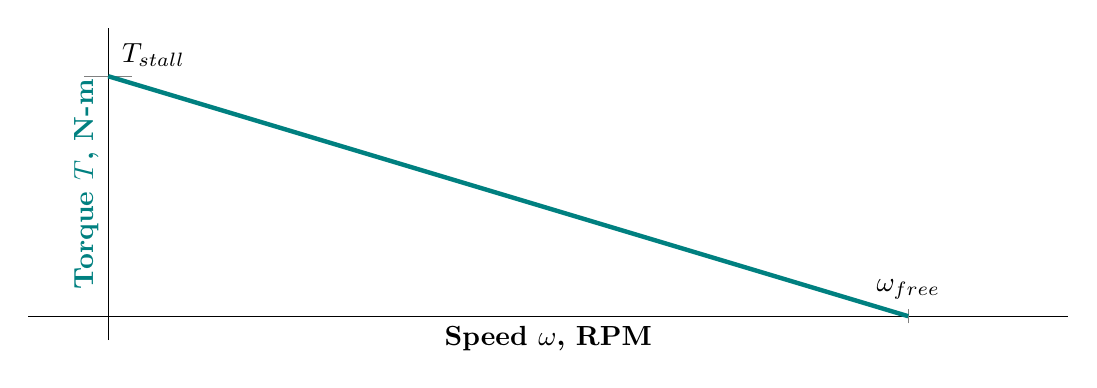
\begin{tikzpicture}[x=4.0in,y=1.2in]
  %\fill[lightgray] (1.0,0)--(0,1.0)--(0,0)--cycle;
  \draw[black] (-0.1,0)--(1.2,0) node[pos=0.5,below]{\bf Speed $\omega$, RPM};
  \draw[black] (0,-0.1)--(0,1.2) node[pos=0.5,above,rotate=90,teal]{\bf Torque $T$, N-m};
  
  \draw[gray] (-0.03,1)--(0.03,1) node[pos=1, above, black]{\bf  \ \ \ \ $T_{stall}$};
  \draw[gray] (1,-0.03)--(1,0.03) node[pos=1, above, black]{\bf $\omega_{free}$};

  \draw[teal, ultra thick] (1.0,0)--(0,1.0);
\end{tikzpicture}
\caption{Torque varies linearly with speed.}
\end{figure}

This could be expressed as an equation for a line,
\begin{align} \label{eq:motor_torque_curve}
  T = T_{stall} \frac{\omega-\omega_{free}}{\omega_{free}}
\end{align}

With the torque and velocity data, we can compute the power; the rate at which torque is done, or

\begin{align} \label{eq:shaft_power}
  P = T \cdot \omega
\end{align}

Substituting Equation \ref{eq:motor_torque_curve} into \ref{eq:shaft_power} yields the following equation for the power curve.

\begin{align} \label{eq:motor_power_curve}
  P = T_{stall} \frac{(\omega_{free}-\omega) \omega}{\omega_{free}}
\end{align}

Note: $\omega$ must be in rad/s, not RPM.

\begin{figure}[H] \centering \label{fig:motor_power_curve}
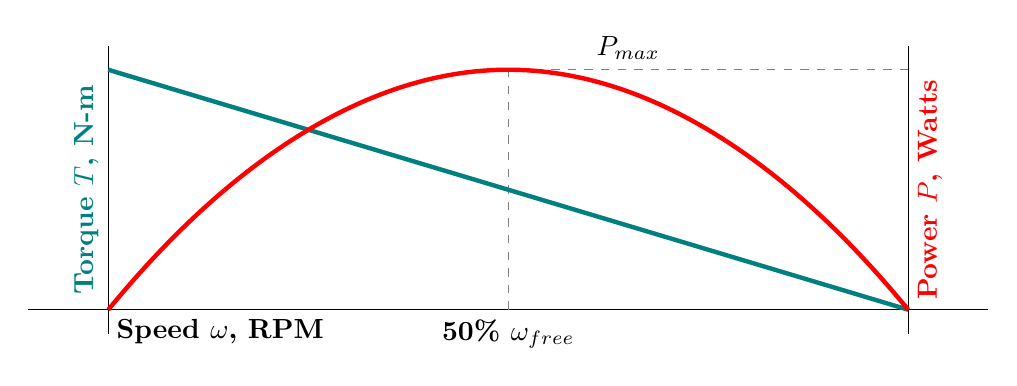
\begin{tikzpicture}[x=4.0in,y=1.2in]
  %\fill[lightgray] (1.0,0)--(0,1.0)--(0,0)--cycle;
  \draw[black] (-0.1,0)--(1.1,0) node[pos=0.2,below]{\bf Speed $\omega$, RPM};
  \draw[black] (0,-0.1)--(0,1.1) node[pos=0.5,above,rotate=90,teal]{\bf Torque $T$, N-m};
  \draw[black] (1,-0.1)--(1,1.1) node[pos=0.5,below,rotate=90,red]{\bf Power $P$, Watts};
  
  \draw[gray, dashed] (0.5, 0) -- (0.5, 1) node[pos=0.0,below, black]{\bf 50\% $\omega_{free}$};
  
  \draw[gray, dashed] (1.0, 1.0) -- (0.5, 1) node[pos=0.7,above, black]{\bf $P_{max}$};

  \draw[teal, ultra thick] (1.0,0)--(0,1.0);
  \draw[red, ultra thick] (0,0) parabola bend (0.5,1.0) (1.0,0.0) ;
\end{tikzpicture}
\caption{Power forms a parabolic curve with speed.}
\end{figure}

From this we can see that the peak power is produced at half of free speed. This is also half of torque.

Current ($I$) is how much electricity is drawn. It varies proportionally to torque, so

\begin{align} \label{eq:motor_current_curve}
  I = C T \nonumber \\
  I = C T_{stall} \frac{\omega_{free}-\omega}{\omega_{free}}
\end{align}

\begin{figure}[H] \centering
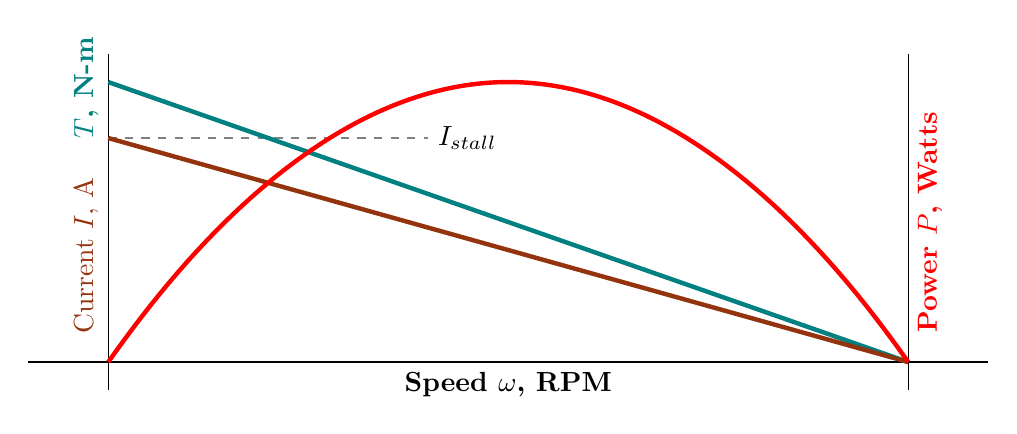
\begin{tikzpicture}[x=4.0in,y=1.4in]
  %\fill[lightgray] (1.0,0)--(0,1.0)--(0,0)--cycle;
  \draw[black] (-0.1,0)--(1.1,0) node[pos=0.5,below]{\bf Speed $\omega$, RPM};
  \draw[black] (0,-0.1)--(0,1.1) node[pos=0.9,above,rotate=90,teal]{\bf $T$, N-m} node[pos=0.4,above,rotate=90,RawSienna]{Current $I$, A};
  \draw[black] (1,-0.1)--(1,1.1) node[pos=0.5,below,rotate=90,red]{\bf Power $P$, Watts};
  
  \draw[gray, dashed] (0, 0.8) -- (0.4, 0.8) node[pos=1,right, black]{\bf $I_{stall}$};

  \draw[teal, ultra thick] (1.0,0)--(0,1.0);
  \draw[RawSienna, ultra thick] (1.0,0)--(0,0.8);
  \draw[red, ultra thick] (0,0) parabola bend (0.5,1.0) (1.0,0.0) ;
\end{tikzpicture}
\caption{Current varies with torque.}
\end{figure}

Efficiency ($\eta$) is a ratio of how much mechanical energy is produced per electrical energy spent.

\begin{equation} \label{eq:motor_efficiency_curve}
  \eta = \frac{P_{mech}}{P_{elec}} = \frac{T-M_{friction} \omega}{V I}
  = \frac{[T_{stall} \ \frac{(\omega_{free}-\omega)}{\omega_{free}} - M_f] \omega}{V\ C\ T_{stall} \frac{(\omega_{free}-\omega)}{\omega_{free}}} \nonumber
\end{equation}

Indeed an ugly equation, let's just plot it with some semi-realistic values.

\begin{figure}[H] \centering
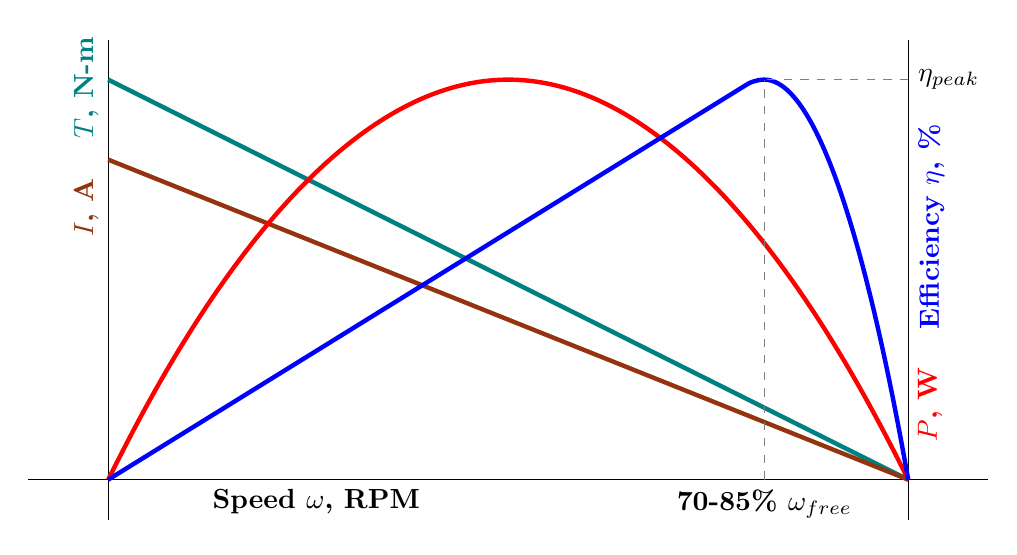
\begin{tikzpicture}[x=4.0in,y=2.0in]
  %\fill[lightgray] (1.0,0)--(0,1.0)--(0,0)--cycle;
  \draw[black] (-0.1,0)--(1.1,0) node[pos=0.3,below]{\bf Speed $\omega$, RPM};
  \draw[black] (0,-0.1)--(0,1.1) node[pos=0.9,above,rotate=90,teal]{\bf $T$, N-m}
  node[pos=0.65,above,rotate=90,RawSienna]{\bf $I$, A};
  \draw[black] (1,-0.1)--(1,1.1) node[pos=0.24,below,rotate=90,red]{\bf $P$, W}
  node[pos=0.61,below,rotate=90,blue]{\bf Efficiency $\eta$, \%};

  \draw[teal, ultra thick] (1.0,0)--(0,1.0);
  \draw[RawSienna, ultra thick] (1.0,0)--(0,0.8);
  \draw[red, ultra thick] (0,0) parabola bend (0.5,1.0) (1.0,0.0) ;
  \draw[blue, ultra thick] (0,0)--(0.8,0.99) parabola bend (0.82,1.0) (1.0,0.0) ;
  
  \draw[gray, dashed] (0.82,0) -- (0.82, 1) node[pos=0,below, black]{\bf 70-85\% $\omega_{free}$};
  
  \draw[gray, dashed] (1,1) -- (0.82, 1) node[pos=0,right, black]{\bf $\eta_{peak}$};
\end{tikzpicture}
\caption{Complete motor curve.}
\end{figure}

In summary:
\begin{asparaitem}
	\item Motors produce less and less torque as they spin up.
	\item No power is produced when the motor is at maximum speed or maximum torque.
	\item Maximum power is produced at 50\% of maximum speed, which is also at 50\% of maximum torque.
	\item Maximum efficiency occurs somewhere between 75\% and 90\% of free speed.
\end{asparaitem}


\section{Comparing Motor Types}

\begin{table}[H]
\begin{tabular}{lll}
                      & \textit{Brushed DC}   & \textit{Brushless DC}                \\
\textbf{Efficiency}            & Low          & High                        \\
\textbf{Mechanical Robustness} & Medium       & High                        \\
\textbf{Electronic Complexity} & Low          & High                        \\
\textbf{Position Control}      & Not inherent & \begin{tabular}[c]{@{}l@{}}May have\\ integrated encoder\end{tabular} \\
\textbf{Cost}                  & Low          & Medium                     
\end{tabular}
\caption{Motor types at a glance}
\end{table}

